\documentclass[UTF8,openany]{book}
\usepackage{ctex} 
\usepackage[hypertexnames=true]{hyperref} 
\usepackage{xcolor}
\usepackage{graphicx,amsfonts,amsmath,mathrsfs,amssymb,amsthm,url,color}
\usepackage{fancyhdr,indentfirst,bm,enumerate,natbib,float,tikz}
\usepackage{caption,subcaption,calligra}
\usepackage{afterpage} 




\let\origcleardoublepage\cleardoublepage
\renewcommand{\cleardoublepage}{\clearpage}

\hypersetup{
	colorlinks=true,
	linkcolor=blue,
	filecolor=magenta,      
	urlcolor=cyan,
	pdftitle={实用随机过程往年卷合集},
	pdfauthor={NULIOUS},
	pdfsubject={主题},
	pdfkeywords={随机过程,往年卷}
}

\title{\Huge 实用随机过程往年卷合集}
\author{\Large \calligra{NULIOUS}}
\date{}

\textheight 23cm
\textwidth 16.5cm
\topmargin -1.2cm
\oddsidemargin 0cm
\evensidemargin 0cm

\begin{document}
\maketitle
\frontmatter 
\begin{center}
	\Huge 前言
\end{center}

{\Large 本文档是实用随机过程往年卷合集,于25年夏天编写,整理了有试题的往年卷的答案,仅供参考,如文档有错误或者有其他问题请发送至我的邮箱\href{mailto:3589851379@qq.com}{3589851379@qq.com}
\vspace{5mm}\\

特别感谢实用随机过程25春的两位助教苏煜庭与华申瑞提供了25期中的解答与25期末的试卷,以及其他分享了往年试题的学长学姐们
\vspace{5mm}\\

我的个人主页:\url{https://mulious.github.io/}

如果本文档里有错误可以先参考原版试卷,原版25,23,19,15年期中有答案:\href{https://github.com/mulious/USTCexam/tree/main/stochastic-processes/original-exam}{实用随机过程往年题原卷}
\vspace{5mm}\\

其他关于本课程的资料可以见pksq链接:\href{https://icourse.club/course/2093/#review-93966}{我的评课}}
\vspace{1cm}
\begin{center}
	\huge 预祝大家在考试前速通成功!
\end{center}
\tableofcontents 
\afterpage{\clearpage}
\mainmatter
\chapter{\centering 往年期中试卷}
\section{\centering 25实用随机过程期中}
\noindent 一、(18分)设 $\{N(t), t \geq 0\}$ 表示一个速率为 $\lambda$ 的 Poisson 过程,而 $S_n$ 为其第 $n$ 个事件的发生时刻,$n \geq 1$。\\
(1) 对任意 $s > 0$,求 $\mathbb{E}[S_2|N(s) = 1]$。\\
(2) 对任意 $s, t > 0$,求协方差 $\operatorname{Cov}(N(s), N(s + t))$。\\
(3) 对任意整数 $n \geq 1$,在 $N(t) = n$ 的条件下,求 $N(2t/3) - N(t/3)$ 的条件分布律。\\
解:\\
\qquad (1)由无记忆性,从 $s$ 时刻开始下次发生的平均时间为 $\displaystyle \frac{1}{\lambda}$,故
\begin{align*}
	\mathbb{E}[S_2 \mid N(s)=1]= s+\frac{1}{\lambda}.
\end{align*}
(2)由独立增量性和协方差的双线性性:
\begin{align*}
	\operatorname{Cov}(N(s),N(s+t)) &= \operatorname{Cov}(N(s),N(s))+\operatorname{Cov}(N(s),N(s+t)-N(s))\\
	&= \operatorname{Var}(N(s))\\
	&= \lambda s.
\end{align*}
(3)
由 $N(t)=n$ 知,$\{S_i,i=1,\dots,n\}$与 $\{U_{(i)},i=1,\dots,n\}$ 同分布,则
$$N(\frac{2}{3}t)-N(\frac{1}{3}t)=k \iff \text{有}\ k\ \text{个}U_i\in(\frac{1}{3}t,\frac{2}{3}t).$$
即为$\displaystyle \mathrm{B}(n,\frac{1}{3})$。\\


\noindent 二、(18分)设在某区间上,轿车,卡车和客车独立地分别以速率 $\lambda_1$, $\lambda_2$ 和 $\lambda_3$ 的 Poisson 过程到达且立即通过。\\
(1) 求所有汽车到达的时间间隔的分布。\\
(2) 设在 $t_0$ 时刻观察到一辆轿车通过,求下一辆通过的汽车仍为轿车的概率。\\
(3) 求在连续两辆轿车通过该路口期间非轿车通过数量的期望。\\
解:\\
(1)由Poisson过程可叠加的性质,汽车到达的过程为Poisson过程 $Poi(\lambda_1+\lambda_2+\lambda_3)$,因此间隔时间分布为 $\mathrm{Exp}(\lambda_1+\lambda_2+\lambda_3)$。\\
(2)设从 $t_0$ 之后下一辆轿车,卡车,客车到达的间隔时间分别为 $X,Y,Z$,由指数分布的无记忆性可得 $X\sim \mathrm{Exp}(\lambda_1),Y\sim \mathrm{Exp}(\lambda_2),Z\sim \mathrm{Exp}(\lambda_3)$,且 $X,Y,Z$ 相互独立,于是
$$
\begin{aligned}
	P(\mbox{下一辆为轿车})&=P(X=\min\{X,Y,Z\})\\&=\int_{0}^\infty \lambda_1e^{-\lambda_1x}e^{-\lambda_2x}e^{-\lambda_3x}dx\\&=\frac{\lambda_1}{\lambda_1+\lambda_2+\lambda_3}.
\end{aligned}
$$
(3)记两次轿车通过之间的时间为 $T\sim \mathrm{Exp}(\lambda_1)$,则由平稳增量性以及三类汽车相互独立可知两次轿车通过之间卡车通过的数量为 $N_2(T)$,客车为 $N_3(T)$,其中 $\{N_2(t)\}$ 和 $\{N_3(t)\}$ 为卡车和客车到达对应的Poisson过程。于是
$$
\begin{aligned}
	\mathbb{E}[N_2(T)+N_3(T)]&=\mathbb{E}[\mathbb{E}[N_2(T)|T]+\mathbb{E}[\mathbb{E}[N_3(T)|T]]\\
	&=\mathbb{E}[\lambda_2T]+\mathbb{E}[\lambda_3T]\\
	&=\frac{\lambda_2+\lambda_3}{\lambda_1}.
\end{aligned}
$$\\


\noindent 三、(12分)设顾客以 $\lambda = 2$ 人每小时的速度到达某个自动取款机,且每个顾客取走的金额相互独立,期望为 $\mu = 500$ 元,方差为 $\sigma^2 = 6000$。以 $X(t)$ 表示到 $t$ 为止顾客取走的总金额(忽略顾客取钱的时间)。求 $X(5)$ 的期望和标准差。\\
解:\\
设第 $i$ 个人取金额 $X_i$,则$$X(t)=\sum_{i=1}^{N(t)}X_i,$$
其中 $N(t) \sim \mathrm{P}(\lambda t),\mathbb{E}[X_i]=\mu,Var(X_i)=\sigma^2$,由复合Poisson过程知,
$$\mathbb{E}[X(t)]=\mathbb{E}[N(t)]\mathbb{E}[X_i],\operatorname{Var}(X(t))=\mathbb{E}[N(t)]\mathbb{E}[X_i^2],$$
故 $\mathbb{E}[X(5)]=\lambda t \cdot \mu=5000,\sqrt{\operatorname{Var}(X(5))}=\sqrt{\lambda t \cdot(\mu^2+\sigma^2)}=1600$。\\


\noindent 四、(12分)设 $\{N(t), t \geq 0\}$ 表示一个速率为 $\lambda$ 的 Poisson 过程,而 $X$ 为一独立于该过程的非负随机变量,且 $\mathbb{E}[X] = \mu$, $\operatorname{Var}(X) = \sigma^2$。求 $\mathbb{E}[N(X)]$ 和 $\operatorname{Var}[N(X)]$。\\
解:\\
利用条件期望平滑公式
$$
\mathbb{E}[N(X)]=\mathbb{E}[\mathbb{E}[N(X)|X]]=\mathbb{E}[\lambda X]=\lambda\mu.
$$
利用条件方差公式
$$
\begin{aligned}
	\operatorname{Var}(N(X))&=\operatorname{Var}(\mathbb{E}[N(X)|X])+\mathbb{E}[\operatorname{Var}(N(X)|X)]\\
	&=\operatorname{Var}(\lambda X)+\mathbb{E}[\lambda X]\\
	&=\lambda^2\sigma^2+\lambda\mu.
\end{aligned}
$$\\


\noindent 五、(20分)考虑一组独立可重复的随机试验,设每次只能出现 A, B 和 C 三种结果之一,且发生的概率依次为 0.5, 0.3 和 0.2。对花样 AAA 和 ABCAB,分别求它们首次出现所需平均试验次数。\\
解:\\
\begin{align*}
	\mathbb{E}[AAA]&=P(A)^{-3}+P(A)^{-2}+P(A)^{-1}\\
	&=14,\\
	\mathbb{E}[ABCAB]&=\mathbb{E}[AB]+P(A)^{-2}P(B)^{-2}P(C)^{-1}\\  &=P(A)^{-1}P(B)^{-1}+P(A)^{-2}P(B)^{-2}P(C)^{-1}\\
	&=\frac{2060}{9}.
\end{align*}\\



\noindent 六、(20分)设 $\{N(t), t \geq 0\}$ 为一更新过程,且其达到间隔时间 $X_1, X_2, \ldots$ 均服从均匀分布 $\mathrm{U}[1, 3]$。\\
(1) 求更新函数 $m(t)$ 的表达式,其中 $0 < t < 3$。\\
(2) 利用关键更新定理求 $\lim_{t \to \infty} \int_0^t e^{-(t-s)} dm(s)$。\\
(3) 设 $Y(t)$ 表示时刻 $t$ 的剩余寿命,求 $\lim_{t \to \infty} \int_0^t Y(s) ds/t$。\\
(4) 求 $\lim_{t \to \infty} \mathbb{E}[Y(t)]$。\\
解:(1)由于间隔时间大于1,于是 $m(t)=0,0<t<1$,当 $t\in[1,2)$ 时,将 $F$ 为 $\mathrm{U}(1,3)$ 的分布函数代入更新方程
$$
\begin{aligned}
	m(t)&=F(t)+\int_{0}^tm(t-x)dF(x)\\
	&=\frac{t-1}{2}+\frac{1}{2}\int_{1}^tm(t-x)dx\\
	&=\frac{t-1}{2}+\frac{1}{2}\int_{0}^{t-1}m(x)dx=\frac{t-1}{2}.
\end{aligned}
$$
当 $t\in[2,3)$ 时
$$
\begin{aligned}
	m(t)&=F(t)+\int_{0}^tm(t-x)dF(x)\\
	&=\frac{t-1}{2}+\frac{1}{2}\int_{1}^tm(t-x)dx\\
	&=\frac{t-1}{2}+\frac{1}{2}\int_{0}^{t-1}m(x)dx\\
	&=\frac{t-1}{2}+\frac{1}{2}\int_{1}^{t-1}\frac{x-1}{2}dx\\
	&=\frac{t-1}{2}+\frac{(t-2)^2}{8}=\frac{t^2}{8}.
\end{aligned}
$$
综上可得
$$
m(t)=
\begin{cases}
	0  &  0<t<1 \\
	\frac{t-1}{2}  &  1\leq t<2\\
	\frac{t^2}{8}  &	2\leq t<3
\end{cases}
$$
(2)令 $h(t)=e^{-t}$,可以验证 $h(t)$ 恒正递减且在 $(0,\infty)$ 上可积$\left( \int_{0}^{+\infty} h(s)ds=1 \right) $,因此满足直接Riemann可积,容易计算间隔时间的期望为2,从而由关键更新定理
$$
\lim_{t\to \infty}\int_{0}^t e^{-(t-s)}dm(s)=\lim_{t\to \infty}\frac{1}{2}\int_{0}^t e^{-s}ds=\frac{1}{2}.$$
(3)记间隔时间对应随机变量为 $X\sim U[1,3]$,由更新报酬过程(课本例3.6B)可得
$$
\lim_{t\to \infty}\frac{\int_{0}^t Y(s)ds}{t}=\frac{\mathbb{E}[X^2]}{2\mathbb{E}[X]}=\frac{13}{12}.
$$
(4)由课本命题3.4.6可得
$$
\lim_{t\to \infty}\mathbb{E}[Y(t)]=\frac{\mathbb{E}[X^2]}{2\mathbb{E}[X]}=\frac{13}{12}.
$$\\
\textbf{RK}:\\
(3)详细过程如下:\\
考虑更新报酬过程,设在$s$时刻收到$Y(s)$的钱
\[
\lim_{t\rightarrow \infty}\frac{\int_{0}^{t} Y(s)ds}{t}=\lim_{t\rightarrow \infty}\frac{\mathbb{E}\left[R(t) \right] }{t}=\frac{\mathbb{E}\left[ R\right] }{\mathbb{E}[X_i]}=\frac{\mathbb{E}\left[R\right] }{2}
\]
另外注意间隔时间$X_n$独立同分布
$$
\begin{aligned}
	\mathbb{E}[R]&=\mathbb{E}\left[\mathbb{E}\left[R\left| X_1=x\right. \right]  \right] \\
	&=\int_{\mathbb{R}} \mathbb{E}[R|X_1=x]f_{x_1}(x)dx\\
	&=\int_{1}^{3} \frac{1}{2}\mathbb{E}[R|X_1=x]dx\\
	&=\frac{1}{2}\int_{1}^{3} \int_{0}^{x}(x-t)dtdx\\
	&=\frac{13}{6}
\end{aligned}
$$
因此
\[
\lim_{t\to \infty}\mathbb{E}[Y(t)]=\frac{13}{12}
\]
(4)详细过程如下
\begin{align*}
	\mathbb{E}[Y(t)]&=\mathbb{E}\left[ Y(t)|S_{N(t)}=0 \right]\bar{F}(t) +
	\int_{0}^{t} \mathbb{E}\left[ Y(t)|S_{N(t)}=y \right]\bar{F}(t-y)dm(y)\\
	&=\mathbb{E}\left[X-t|X>t \right]\bar{F}(t)+ 	\int_{0}^{t} \mathbb{E}\left[X-(t-y)|X>t-y \right]\bar{F}(t-y)dm(y)\\
\end{align*}
设$h(t)=\mathbb{E}\left[X-t|X>t \right]\bar{F}(t)$,则其非负不增,且$\int_{0}^{+\infty} h(t)dt<\infty$(见下面计算过程)\\
由关键更新定理
\[
\lim_{t\to \infty}\mathbb{E}[Y(t)]=0+\frac{1}{\mu}\int_{0}^{+\infty}h(t)dt
\]
这里用到了$\lim_{t\to \infty}\bar{F}(t)=0$\\
由期望的定义(这里将密度$f_{X|X>t}(s)$改写为$P(X=s|X>t)$)
$$
\begin{aligned}
	\mathbb{E}\left[X-t|X>t \right]\bar{F}(t)&=\int_{t}^{+\infty}(s-t) f_{X|X>t}(s)P(X>t)ds\\
	&=\int_{t}^{+\infty}(s-t) P(X=s|X>t)P(X>t)ds\\
	&=\int_{t}^{+\infty} (s-t)P(X=s,X>t)ds\\
	&=\int_{t}^{+\infty} (s-t)dF(s)\\
	&\left( =\mathbb{E}\left[(X-t) \mathbb{I}_{\{X >t\}}\right]\right)  
\end{aligned}
$$
上式也可以由全概率公式(对$X$的取值取条件)得到
$$
\begin{aligned}
	\mathbb{E}\left[X-t|X>t \right]\bar{F}(t)&=\int_{t}^{+\infty}\mathbb{E}\left[X-t|X>t,X=s \right] P(X>t|X=s)P(X=s)ds\\
	&=\int_{t}^{+\infty} (s-t)P(X=s,X>t)ds\\
	&=\int_{t}^{+\infty} (s-t)dF(s)\\
	&\left( =\mathbb{E}\left[(X-t) \mathbb{I}_{\{X >t\}}\right]\right)  
\end{aligned}
$$
则
$$
\begin{aligned}
	\lim_{t\to \infty}\mathbb{E}[Y(t)]&=\frac{1}{\mu}\int_{0}^{+\infty} \int_{t}^{\infty}(s-t)dF(s)dt\\
	&\stackrel{Fubini\text{换序}}{=}\frac{1}{\mu}\int_{0}^{+\infty} \int_{0}^{s}(s-t)dtdF(s)\\
	&=\frac{\mathbb{E}[X_i^2]}{2\mu}\\
	&=\frac{13}{12}
\end{aligned}
$$\\



\noindent 七、(附加题, 10分)设 $\{N_D(t), t \geq 0\}$ 为一延迟更新过程,且其达到间隔时间 $X_1$ 和 $X_2$ 分别服从参数为 $\lambda$ 和 $\mu$ 的指数分布。试求更新函数 $m_d(t)$ 的精确表达式。\\
解:\\
我们先不看延迟更新的部分(当作$X_1=0$),先求解后半部分(普通更新过程$N(t)$)的更新函数$m(t)$\\
法一:\\
注意Poisson过程可以由如下定义:\\
设$\{X_n\}\stackrel{i.i.d.}{\sim} \mathrm{Exp}(\lambda)$,第$n$个事件发生的时刻$S_n$为
\[
S_n=X_1+X_2+\dots+X_n
\]
这样定义的计数过程为速率为$\lambda$的Poisson过程\\
则本题的延迟更新过程实际上是一个指数分布加上一个参数为$\mu$的Poisson过程$N(t)$\\
对于Poisson过程$N(t)$,它的更新函数为
\[
m(t)=\mathbb{E}[N(t)]=\mu t
\]
法二:\\
设 $X_1\sim F,X_2\sim G$,
记 $m(t)=\sum_{n=1}^{\infty}G_n(t)$,则有更新方程
\begin{align*}
	m(t)&=G(t) + \int_0^t m(t - x) dG(x)\\
	&=1-e^{-\mu t}+\int_0^t m(t - x)  \mu e^{-\mu x}dx\\
	&=1-e^{-\mu t}+\int_0^t m(x)  \mu e^{-\mu (t-x)}dx\\
	&=1-e^{-\mu t}+\mu e^{-\mu t}\int_0^t m(x)e^{\mu x}dx\\
	\Rightarrow m'(t)&=\mu e^{-\mu t}+\mu m(t)+\int_0^t m(x)e^{\mu x}dx\cdot(-\mu^2e^{-\mu t})\\
	&=\mu e^{-\mu t}+\mu m(t)+(-\mu)\cdot(m(t)-1+e^{-\mu t})\\
	&=\mu
\end{align*}
代入$\mathbb{E}[N(t)]=m(0)=0$,有
\[
m(t)=\mathbb{E}[N(t)]=\mu t
\]
再计算延迟更新过程的更新函数$m_d(t)$\\
法一:\\
利用延迟更新过程的更新方程
\begin{align*}
	m_d(t)&=F(t)+\sum_{n=1}^{\infty}G_n(t)*F(t)\\
	&=F(t)+\int_0^t m(t - x) dF(x)\\
	&=1-e^{-\lambda t}+\int_0^t \mu (t - x) \lambda e^{-\lambda x}dx\\
	&=1-e^{-\lambda t}+\mu t+\frac{\mu}{\lambda}e^{-\lambda t}-\frac{\mu}{\lambda}.
\end{align*}
法二:\\
对首次更新发生的时刻$s$取条件
$$
m_d(t)=\mathbb{E}[N_D(t)]=\mathbb{E}\left[\mathbb{E}[N_D(t)|X_1=s] \right] 
$$
且有
$$
\mathbb{E}[N_D(t)|X_1=s]=
\begin{cases}
	1+\mathbb{E}[N(t-s)]  &  t>s \\
	0  &  t\le s
\end{cases}
$$
则
$$
\begin{aligned}
	m_d(t)=\mathbb{E}[N_D(t)]&=\int_{0}^{t} \left(1+\mathbb{E}[N(t-s)] \right) \lambda e^{-\lambda s}ds\\
	&=\int_{0}^{t} \left(1+\mu(t-s) \right) \lambda e^{-\lambda s}ds\\
	&=(1+\mu t)\left(-e^{-\lambda t}+1 \right) -\mu \int_{0}^{t} s\lambda e^{-\lambda s}ds \\
	&=(1+\mu t)\left(-e^{-\lambda t}+1 \right) -\frac{\mu}{\lambda}\left( -\lambda t e^{-\lambda t} -e^{-\lambda t}+1\right)\\
	&=1-e^{-\lambda t}+\mu t+\frac{\mu}{\lambda}e^{-\lambda t}-\frac{\mu}{\lambda}
\end{aligned}
$$
\newpage
\section{\centering 24实用随机过程期中}
\noindent 1.(20 分)系统有两个编号为 1,2 的服务台,第 $i$ 号服务台给顾客提供的服务时间服从失效率为常数 $\lambda_{i}$ 的指数分布,其中 $i=1,2$ ,不同顾客的服务时间相互独立.采用先到先服务、后到排队的原则。当 A 到达系统时,发现 B 和 C 占据了两个服务台,求 A 在系统中滞留时间 $T$ 的期望.\\
解:利用指数分布的性质
\[
X_1\sim \mathrm{Exp}(\lambda_1) \quad X_2\sim \mathrm{Exp}(\lambda_2) 
\]
则有
\[
P(X_1<X_2)=\frac{\lambda_1}{\lambda_1+\lambda_2}
\]
和
\[
\min\{X_1,X_2\} \sim \mathrm{Exp}(\lambda_1+\lambda_2)
\]
设顾客$B$与$C$的服务时长分别为$X_1$与$X_2$,则
\begin{align*}
	\mathbb{E}\left[\text{顾客A在系统中滞留的时间} \right]  &= \mathbb{E}\left[\text{顾客A在系统中滞留的时间}\mid \text{B比C先走} \right]P(\text{B比C先走})\\
	&+\mathbb{E}\left[\text{顾客A在系统中滞留的时间}\mid \text{C比B先走} \right]P(\text{C比B先走}) \\
	& = \left(\frac{1}{\lambda_1+\lambda_2}+\frac{1}{\lambda_1} \right)\cdot \frac{\lambda_1}{\lambda_1+\lambda_2}+ \left(\frac{1}{\lambda_1+\lambda_2}+\frac{1}{\lambda_2} \right)\cdot \frac{\lambda_2}{\lambda_1+\lambda_2}\\
	&=\frac{3}{\lambda_1+\lambda_2}
\end{align*}\\


\noindent 2.(每小题 6 分,总 24 分)考虑一个 $M / G / \infty$ 系统,顾客到达系统的规律可以用齐次 Poisson 过程来描述,单位时间内平均到达的顾客数为 5 ,每个顾客需要服务员提供的服务时间相互独立,服从区间 $(1,3)$ 上的均匀分布,系统有无穷多个服务员(即顾客到达系统后立即能得到服务)\\
(1)求于 $(0,4]$ 到达,且于时刻 5 未被服务完毕的顾客人数 $M_{1}$ 服从的分布;\\
(2)求于 $(0,4]$ 到达,且于 $(4,5]$ 内被服务完毕的顾客人数 $M_{2}$ 服从的分布;\\
(3)求于 $(3,4]$ 到达,且于时刻 5 末被服务完毕的顾客人数 $M_{3}$ 服从的分布;\\
(4)判断 $M_{1}, M_{2}, M_{3}$ 两两之间的独立性.\\
解:(1)服务时间$G$的密度为
\[
g(x)=
\begin{cases}
	\frac{1}{2}  &  1<x<3 \\
	0  &  \text{其他}
\end{cases}
\]
其分布函数为
\[
G(x)=
\begin{cases}
	1  &  x<1 \\
	\frac{x-1}{2}  &  1\le x\le 2\\
	0  &  x>2 
\end{cases}
\]
则服务时间的生存函数为
\[
\bar{G}(x)=1-G(x)=
\begin{cases}
	0  &  x<1 \\
	\frac{3-x}{2}  &  1\le x\le 2\\
	1  &  x>2 
\end{cases}
\]
于 $(0,4]$ 中$s$时刻到达,且于时刻 5 未被服务完毕的概率为
\[
P_1(s)=
\begin{cases}
	\bar{G}(5-s) &  s\le 4 \\
	0  &  s > 4
\end{cases}
=
\begin{cases}
	\frac{s-2}{2} & 2\le s\le 4 \\
	0  &  \text{其他}
\end{cases}
\]
则由分类Poisson过程有
\[
M_1 \sim \mathrm{P}\left(\lambda \int_{0}^{5} P_1(s)ds  \right) =\mathrm{P}(5)
\]
(2)于 $(0,4]$ 中$s$时刻到达,且于$(4,5]$内被服务完毕的概率为
\[
P_2(s)=
\begin{cases}
	1  &  0<s\le 2 \\
	G(5-s)  &  2<s\le 4\\
	0 & s>4
\end{cases}
=
\begin{cases}
	1  &  0<s\le 2 \\
	\frac{4-s}{2}  &  2<s\le 4\\
	0 & s>4
\end{cases}
\]
则由分类Poisson过程有
\[
M_2 \sim \mathrm{P}\left(\lambda \int_{0}^{5} P_2(s)ds  \right) =\mathrm{P}(15)
\]
(3)于 $(3,4]$ 中$s$时刻 到达,且于时刻 5 末被服务完毕的概率为
\[
P_3(s)=
\begin{cases}
	0  &  s\le 3 \\
	\bar{G}(5-s)  &  3<s\le 4\\
	0 & s>4
\end{cases}
=
\begin{cases}
	0  &  s\le 3 \\
	\frac{s-2}{2}  &  3<s\le 4\\
	0 & s>4
\end{cases}
\]
则由分类Poisson过程有
\[
M_3 \sim \mathrm{P}\left(\lambda \int_{0}^{5} P_3(s)ds  \right) =\mathrm{P}\left(\frac{15}{4} \right) 
\]
(4)由分类Poisson过程,$M_1$和$M_2$是独立的,$M_2$和$M_3$也是独立的,而$M_1$和$M_3$不是独立的,因为原Poisson过程$N(t)$中的$N(4)$和$N(4)-N(3)$不是独立的\\





\noindent 3.(每小题 4 分,总 16 分)假设一个元件于时刻 0 开始投入使用,该元件易于受到外界的冲击,时间单位按小时计算.在时间段 $(0,3]$ 内冲击以每小时 2 个的泊松速率到达,在时间段 $(3,6]$ 内冲击以每小时 3 个的泊松速率到达,在其后的时间段 $(6,+\infty)$ 内冲击以每小时 1 个泊松速率到达.泊松速率到达是指不可能有两个或多个冲击同时到达.\\
(1)问冲击到达可以用什么样的过程来描述?\\
(2)求时间段 $(2,4]$ 有 1 个冲击发生的概率.\\
(3)求时间段 $(2,4]$ 和 $(4,6]$ 中各有 1 个冲击发生的概率.\\
(4)求前 10 个小时之内到达冲击期望个数\\
解:(1)这是一个非齐次Poisson过程$N(t)$,有强度函数
\[
\lambda(t)=
\begin{cases}
	2  &  0<t\le 3 \\
	3  &  3<t\le 6 \\
	1  &  t>6
\end{cases}
\]
(2)
\[
N(4)-N(2)\sim \mathrm{P}\left(\int_{2}^{4}\lambda(s)ds \right)=\mathrm{P}(5) 
\]
则
\[
P(N(4)-N(2)=1)=5e^{-5}
\]
(3)由独立增量性,两个事件是独立的,且
\[
N(6)-N(4)\sim \mathrm{P}\left(\int_{4}^{6}\lambda(s)ds \right)=\mathrm{P}(6) 
\]
则
\begin{align*}
	P(N(4)-N(2)=1,N(6)-N(4)=1) &= P(N(4)-N(2)=1) P(N(6)-N(4)=1)\\
	& =30e^{-11}
\end{align*}
(4)
\[
N(10)\sim \mathrm{P}\left(\int_{0}^{10}\lambda(s)ds \right)=\mathrm{P}(19) 
\]
则
\[
\mathbb{E}[N(10)]=19
\]\\



\noindent 4.(16 分)以 $A(t)$ 和 $Y(t)$ 记一个更新过程在时刻 $t$ 的年龄和剩余寿命,且假设更新间隔服从参数为 $\lambda$ 的指数分布,求 $\mathrm{P}(Y(t)>x \mid A(t+x)>s)$ ,其中 $s<t+x$ .\\
解:\\
i.$s<x$时\\
$A(t+x)>s$说明$(t+x-s,t+x)$时间段内不可能发生更新,则利用指数分布的无记忆性和生存函数$$\bar{F}(x)=e^{-\lambda x}$$
有
\begin{align*}
	\mathrm{P}(Y(t)>x \mid A(t+x)>s) & =P\left( (t,t+x)\text{时间段内不发生更新}\mid (t+x-s,t+x)\text{时间段内不发生更新}\right)  \\
	& = \frac{ P\left( (t,t+x)\text{时间段内不发生更新}, (t+x-s,t+x)\text{时间段内不发生更新}\right)}{ P\left(  (t+x-s,t+x)\text{时间段内不发生更新}\right)}\\
	&=\frac{ P\left( (t,t+x)\text{时间段内不发生更新}\right)}{ P\left(  (t+x-s,t+x)\text{时间段内不发生更新}\right)}\\
	&=\frac{\bar{F}(x)}{\bar{F}(s)}\\
	&=e^{-\lambda (x-s)}
\end{align*}
ii.$x\le s<t+x$时\\
$A(t+x)>s$就说明在时刻$t+s$距离上一次更新的时间间隔大于$s$,也就大于$x$,所以$(t,t+x)$时间段内不可能发生更新,这就说明$t$时刻距离下一次更新的时间间隔大于$x$,即$Y(t)>x$必然发生
\[
\mathrm{P}(Y(t)>x \mid A(t+x)>s)=1
\]
\textbf{RK}:更新间隔服从参数为 $\lambda$ 的指数分布的更新过程事实上就是参数为 $\lambda$ 的Poisson过程\\



\noindent 5.(每小题6分,总24分)观察一列独立同分布的离散随机变量序列 $\left\{W_{n}, n \geq 1\right\}$ ,已知
$$
\mathrm{P}\left(W_{1}=0\right)=\frac{1}{6}, \quad \mathrm{P}\left(W_{1}=1\right)=\frac{1}{3}, \quad \mathrm{P}\left(W_{1}=2\right)=\frac{1}{2}
$$
(1)分别求等待花样$"121"$和花样$"212"$首次发生所需要的期望时间.\\
(2)给定花样$"121"$已发生,求等待花样$"212"$首次发生所需要的额外期望时间.\\
(3)求等待花样$"121"$或花样$"212"$首次发生所需要的期望时间.\\
(4)求花样$"121"$于花样$"212"$之前发生的概率.\\
解:花样问题\\
(1)"121"有重叠"1","1"没有重叠;"212"有重叠"2","2"没有重叠,则
\[
\mathbb{E}[N_{121}]=\left( P^2\left(W_{1}=1\right)P\left(W_{1}=2\right) \right)^{-1} +\left(P\left(W_{1}=1\right) \right)^{-1}=21
\]
\[
\mathbb{E}[N_{212}]=\left(P\left(W_{1}=1\right)P^2\left(W_{1}=2\right) \right)^{-1} +\left(P\left(W_{1}=2\right) \right)^{-1}=14
\]
(2)花样$"121"$给花样$"212"$提供了花样$"21"$,并注意到"21"没有重叠,因此
\[
\mathbb{E}[N_{212\mid 121}]=\mathbb{E}[N_{212}]-\mathbb{E}[N_{21}]=21-6=15
\]
类似的,花样$"212"$给花样$"121"$提供了花样$"12"$,并注意到"12"没有重叠,因此
\[
\mathbb{E}[N_{121\mid 212}]=\mathbb{E}[N_{121}]-\mathbb{E}[N_{12}]=14-6=8
\]
(3)+(4)设$P_A=P(\text{花样$"121"$于花样$"212"$之前发生})$,$M=\min(N_{121},N_{212})$\\
对花样$"121"$是否于花样$"212"$之前发生取条件,有
\begin{align*}
	\mathbb{E}[N_{121}] & =\mathbb{E}[M]+\mathbb{E}[N_{121}-M] \\
	& = \mathbb{E}[M]+\mathbb{E}[N_{121}-M\mid \text{花样$"121"$于花样$"212"$之前发生}](1-P_A)\\
	&=\mathbb{E}[M]+\mathbb{E}[N_{121\mid 212}](1-P_A)
\end{align*}
类似的
\[
\mathbb{E}[N_{212}]=\mathbb{E}[M]+\mathbb{E}[N_{212\mid 121}]P_A
\]
最后
\[
P_A=\frac{\mathbb{E}[N_{212}]+\mathbb{E}[N_{121\mid 212}]-\mathbb{E}[N_{121}]}{\mathbb{E}[N_{212\mid 121}]+\mathbb{E}[N_{121\mid 212}]}=\frac{1}{23}
\]
\[
\mathbb{E}[M]=\mathbb{E}[N_{212}]-\mathbb{E}[N_{212\mid 121}]P_A=\frac{307}{23}
\]
\newpage
\section{\centering 23实用随机过程期中}
\noindent 1.(总 18 分,每小题 6 分)设顾客到达某个商店的规律可以用参数 $\lambda=1$ 的齐次 Poisson过程 $\{N(t), t \geq 0\}$ 来描述,时间单位为小时.已知前 1 个小时内仅有 2 位顾客到达.\\
(1)求第 2 个小时内有 3 位顾客到达的概率;\\
(2)求这 2 位顾客都是在前 20 分钟到达的概率;\\
(3)求至少有一位顾客是在前 20 分钟到达的概率.\\
解:(1)利用独立增量性质得
$$
P(N(2)-N(1)=3 \mid N(1)=2)=P(N(2)-N(1)=3)=\frac{1}{6} \lambda^{3} e^{-\lambda}=\frac{1}{6 e}
$$
(2)+(3) 利用 $\left[\left(S_{1}, S_{2}\right) \mid N(1)=2\right] \stackrel{d}{=}\left(U_{(1)}, U_{(2)}\right)$ ,其中 $U_{1}, U_{2}$ iid $\sim \mathrm{U}(0,1)$, $\left(U_{(1)}, U_{(2)}\right)$为其次序统计量,于是,
$$
\begin{gathered}
	P\left(S_{1} \leq \frac{1}{3}, \left.S_{2} \leq \frac{1}{3} \right\rvert\, N(1)=2\right)=P\left(U_{1} \leq \frac{1}{3}, U_{2} \leq \frac{1}{3}\right)=\frac{1}{9} \\
	P\left(\left.S_{1} \leq \frac{1}{3} \right\rvert\, N(1)=2\right)=1-P\left(U_{1}>\frac{1}{3}, U_{2}>\frac{1}{3}\right)=\frac{5}{9}
\end{gathered}
$$\\


\noindent 2.(15 分)设 $\{N(t), t \geq 0\}$ 是参数为 $\lambda=1$ 的齐次 Poisson 过程,事件发生时刻序列记为 $\left\{S_{n}, n \geq 1\right\}$ .求
$$
\mathbb{E}\left[\sum_{k=1}^{N(\pi / 2)} \sin \left(S_{k}\right)\right], \quad \operatorname{Var}\left(\sum_{k=1}^{N(\pi / 2)} \sin \left(S_{k}\right)\right)
$$\\
解:设 $\left\{U_{k}, k \geq 1\right\} \mathrm{iid} \sim \mathrm{U}(0, \pi / 2)$ ,则
$$
\sum_{k=1}^{N(\pi / 2)} \sin \left(S_{k}\right) \stackrel{d}{=} \sum_{k=1}^{N(\pi / 2)} \sin \left(U_{k}\right)
$$
上式来自有限求和可以交换次序;并注意到右端为复合 Poisson 过程。于是
$$
\begin{gathered}
	\mathbb{E}\left[\sum_{k=1}^{N(\pi / 2)} \sin \left(S_{k}\right)\right]=\frac{\lambda \pi}{2} \mathbb{E}\left[\sin \left(U_{1}\right)\right]=\lambda=1 \\
	\operatorname{Var}\left(\sum_{k=1}^{N(\pi / 2)} g\left(S_{k}\right)\right)=\frac{\lambda \pi}{2} \mathbb{E}\left[g^{2}\left(U_{1}\right)\right]=\lambda \int_{0}^{\pi / 2} \sin ^{2} x d x=\frac{\lambda \pi}{4}=\frac{\pi}{4}
\end{gathered}
$$\\


\noindent 3.(总 38 分,前 3 题每小题 6 分,后 2 小题每题 10 分)假设冲击按参数为 $\lambda=1$ 的 Poisson 过程发生,且假设每次冲击独立地以概率 $p$ 引起系统失效。以 $M_{r}$ 记使得系统第 $r$ 次失效的冲击数,$T_{r}$ 表示系统第 r 次失效的时刻,其中 $r \geq 1$ 为整数。\\
(1)求 $M_{2}$ 的概率分布;\\
(2)给定 $M_{2}=n \geq 2$ ,求 $T_{2}$ 的条件分布;\\
(3)求 $\mathrm{P}\left(M_{2}=n \mid T_{2}=t\right)$ ,其中 $n \geq 2$ ;\\
(4)求 $\mathrm{P}\left(M_{r}=n \mid T_{r}=t\right)$ ,其中 $n \geq r \geq 3$ ;\\
(5)假设每次冲击造成系统的损失为 $c_{1}$ 元,若造成系统失效,则还需要额外的 $c_{2}$ 元维修损失费.记 $R(t)$ 为 $(0, t]$ 时间段冲击造成系统总的损失费,求 $\lim _{t \rightarrow \infty} R(t) / t$ .\\
解:(1)首先,$M_{2} \sim \mathrm{NB}(2, p)$服从参数为 $(2 . p)$ 的负二项分布,取值于 $\{2,3, \ldots\}$ ,即
$$
P\left(M_{2}=n\right)=\binom{n-1}{1} p^{2}(1-p)^{n-2}=(n-1) p^{2}(1-p)^{n-2}, \quad n \geq 2
$$
(2)利用 $\left[T_{2} \mid M_{2}=n\right]=\left[S_{n} \mid M_{2}=n\right]=S_{n} \sim \Gamma(n, 1)$ .\\
\textbf{RK}:$n$个独立的指数分布$X_i \sim \mathrm{Exp}(\lambda),i=1,...,n$,则其独立和$\sum_{i=1}^n X_i \sim \Gamma\left(n,\lambda \right) $\\
(3)可以参考(4)中的一般解法\\
记 $g_{T_{2} \mid M_{2}}(t \mid n)$ 为 $\left[T_{2} \mid M_{2}=n\right]$ 的条件概率密度函数,则由(2)得
$$
g_{T_{2} \mid M_{2}}(t \mid n)=\frac{\lambda(\lambda t)^{n-1}}{(n-1)!} e^{-\lambda t}
$$
对 $M_{2}$ 取条件,由(2)可以得到 $T$ 的概率密度函数为
$$
\begin{aligned}
	g_{T_{2}}(t) & =\sum_{k=2}^{\infty} g_{T_{2} \mid M_{2}}(t \mid k) \cdot P\left(M_{2}=k\right) \\
	& =\sum_{k=2}^{\infty} \frac{\lambda(\lambda t)^{k-1}}{(k-1)!} e^{-\lambda t} \cdot(k-1) p^{2}(1-p)^{k-2}=p^{2} \lambda^{2} t e^{-\lambda t p}
\end{aligned}
$$
于是,当 $n \geq 2$ 时,
$$
P\left(M_{2}=n \mid T_{2}=t\right)=\frac{g_{T_{2} \mid M_{2}}(t \mid n) \cdot \mathrm{P}\left(M_{2}=n\right)}{g_{T_{2}}(t)}=\frac{[\lambda t(1-p)]^{n-2}}{(n-2)!} \exp \{-\lambda t(1-p)\}
$$
(4)考虑 Poisson 过程事件分类,任意时刻 $s$ 发生的冲击事件以概率 $p$ 划为 I 型事件(造成系统失效),以概率 $1-p$ 划为 II 型事件(未造成系统失效),分别以 $N_{i}(t)$表示 $(0, t]$ 时间段 $i$ 型事件发生的个数,则$N_1(t),N_2(t)$相互独立。给定 $T_{r}=t$ 表示系统于时刻 $t$ 第 $r$ 次失效,且第 $r$ 个 I型事件一定发生于时刻 $t$ ,截止到$t$时刻的 所有冲击个数应该为 $M_r=N_{2}(t)+r$ ,即
$$
\left[M_{r}-r \mid T_{r}=t\right]=N_{2}(t) \sim \operatorname{Poi}(\lambda t(1-p))
$$
于是,
$$
P\left(M_{r}=n \mid T_{r}=t\right)=\mathrm{P}\left(N_{2}(t)=n-r \right)=\frac{[\lambda(1-p) t]^{n-r}}{(n-r)!} \exp \{-\lambda(1-p) t\}
$$
(5)引进一个更新酬劳过程,每当冲击造成系统失效,则称一个更新发生,该时刻称为更新点。此时,一个更新间隔长度 $T$ 与 $T_{1}$ 同分布,一个更新间隔里总的酬劳 $R$ 与 $c_{1} M_{1}+c_{2}$ .注意到$M_1 \sim \mathrm{Ge}(p)$,则
$$
\mathbb{E}\left[T_{1}\right]=\mathbb{E}\left[\sum_{i=1}^{M_{1}} X_{i}\right]=\mathbb{E}\left[ \mathbb{E}\left[\sum_{i=1}^{M_{1}} X_{i}\mid M_1\right]\right] =\frac{1}{\lambda}\mathbb{E}[M_1]=\frac{1}{\lambda p} 
$$
$$
\mathbb{E}[R]=c_{1} \mathbb{E}\left[M_{1}\right]+c_{2}=\frac{c_{1}}{p}+c_{2}
$$
其中 $\left\{X_{k}\right\}$ 为冲击到达间隔.于是,利用更新酬劳过程理论得
$$
\lim _{t \rightarrow \infty} \frac{R(t)}{t}=\frac{\mathbb{E}\left[T_{1}\right]}{\mathbb{E}[R]}=c_{1} \lambda+c_{2} \lambda p=c_{1}+c_{2} p
$$\\



\noindent 4.(14 分)设一个元件的工作过程可以用更新过程 $\{N(t), t \geq 0\}$ 来描述,更新间隔序列 $\left\{X_{n}, n \geq 1\right\}$ 独立同分布,共同分布 $F$ 具有非格子点性质,且满足 $\mathbb{E}\left[X_{1}\right]=1$ , $\mathbb{E}\left[X_{1}^{3}\right]=3$ ,记 $Y(t)$ 为元件于时刻 $t$ 的剩余寿命,求 $\lim _{t \rightarrow \infty} {\mathbb{E}}\left[Y^{2}(t)\right]$ .\\
证法一:记 $h(t)=\mathbb{E}\left[(X-t)^{2}\mid X>t\right]\bar{F}(t)$ ,其中 $X \sim F$ .对 $t$之前最后一次更新发生时刻 $S_{N(t)}$ 取条件得
$$
\begin{aligned}
	\mathbb{E}\left[Y^{2}(t)\right]= & \mathbb{E}\left[Y^{2}(t) \mid S_{N(t)}=0\right] \cdot \bar{F}(t) \\
	& +\int_{0}^{t} \mathbb{E}\left[Y^{2}(t) \mid S_{N(t)}=y\right] \bar{F}(t-y) \mathrm{d} m(y) \\
	= & \mathbb{E}\left[(X-t)^{2} \mid X>t\right] \bar{F}(t) \\
	& +\int_{0}^{t} \mathbb{E}\left[(X-(t-y))^{2} \mid X>t-y\right] \bar{F}(t-y) \mathrm{d} m(y) \\
	= & h(t)+\int_{0}^{t} h(t-y) \mathrm{d} m(y) 
\end{aligned}
$$
由关键更新定理,并注意到$\bar{F}(t)\rightarrow 0 (t\rightarrow \infty)$,则有
$$
\begin{aligned}
	\lim _{t \rightarrow \infty} {\mathbb{E}}\left[Y^{2}(t)\right]&=0+\frac{1}{\mu}\int_{0}^{\infty}h(t)dt\\
	&=\frac{1}{\mu}\int_{0}^{\infty} \mathbb{E}\left[(X-t)^2\mid X >t\right]\bar{F}(t)dt 
\end{aligned}
$$
由期望的定义(这里将密度$f_{X|X>t}(s)$改写为$P(X=s|X>t)$)
\begin{align*}
	\mathbb{E}\left[(X-t)^2\mid X >t\right]\bar{F}(t) &
	=\int_{t}^{\infty} (s-t)^2 f_{X|X>t}(s)P(X>t)ds  \\ &=\int_{t}^{\infty} (s-t)^2 P(X=s|X>t)P(X>t)ds  \\
	& = \int_{t}^{\infty} (s-t)^2 P(X=s , X>t)ds  \\
	& = \int_{t}^{\infty}  (s-t)^2 dF(s)\\
	&\left( =\mathbb{E}\left[(X-t)^2 \mathbb{I}_{\{X >t\}}\right]\right) 
\end{align*}
上式也可以由全概率公式(对$X$的取值取条件)得到
\begin{align*}
	\mathbb{E}\left[(X-t)^2\mid X >t\right]\bar{F}(t) & =\int_{t}^{\infty} \mathbb{E}\left[(X-t)^2 \mid X=s,X>t \right] P(X>t \mid X=s)P(X=s)ds  \\
	& = \int_{t}^{\infty} (s-t)^2 P(X=s , X>t)ds  \\
	& = \int_{t}^{\infty}  (s-t)^2 dF(s)\\
	&\left( =\mathbb{E}\left[(X-t)^2 \mathbb{I}_{\{X >t\}}\right]\right) 
\end{align*}
最后
\begin{align*}
	\lim _{t \rightarrow \infty} {\mathbb{E}}\left[Y^{2}(t)\right]&=\frac{1}{\mu}\int_{0}^{\infty} \int_{t}^{\infty} (s-t)^2dF(s)dt\\
	& \stackrel{Fubini\text{换序}}{=}\frac{1}{\mu}\int_{0}^{\infty} \int_{0}^{s} (s-t)^2dtdF(s)\\
	& =\frac{1}{\mu} \int_{0}^{\infty} \frac{s^3}{3}dF(s)\\
	&=\frac{\mathbb{E}\left[X_1^3  \right]}{3\mu}\\
	&=1
\end{align*}
\textbf{RK}:把过程中的$2$换成$r\in \mathbb{Z}^+$,结论类似地成立,即\\
$$
\lim _{t \rightarrow \infty} {\mathbb{E}}\left[Y^{r}(t)\right]=\frac{\mathbb{E}\left[X_1^{r+1} \right]}{(r+1)\mu}
$$
证法二:对首次更新发生时刻 $X_{1}$ 取条件,得
$$
\mathbb{E}\left[Y^{2}(t)\right]=\mathbb{E}\left[Y^{2}(t) \mid X_{1}>t\right] \cdot \bar{F}(t)+\int_{0}^{t} \mathbb{E}\left[Y^{2}(t) \mid X_{1}=y\right] d F(y)
$$
记 $h(t)=\mathbb{E}\left[(X-t)_{+}^{2}\right], g(t)=\mathbb{E}\left[Y^{2}(t)\right]$ ,则
$$
g(t)=h(t)+\int_{0}^{t} g(t-y) \mathrm{d} F(y)
$$
因此,
$$
g(t)=h(t)+\int_{0}^{t} h(t-y) \mathrm{d} m(y)
$$
余下同证法一.\\



\noindent 5.(15 分)观察一列独立同分布的离散随机变量 $W_{1}, W_{2}, \ldots$ ,等待花样" 22322 "的发生.设
$$
\mathrm{P}\left(W_{1}=0\right)=\mathrm{P}\left(W_{1}=1\right)=\frac{1}{8}, \quad \mathrm{P}\left(W_{1}=2\right)=\frac{1}{2}, \quad \mathrm{P}\left(W_{1}=3\right)=\frac{1}{4}
$$
求等待花样" 22322 "首次发生所需要的期望时间.\\
解法一:构造标准更新酬劳过程 $\left\{X_{n}, n \geq 1\right\}$ 如下:首次出现的花样" 22322 "时刻称为首次更新时刻:从该时刻以后开始(不考虑该时刻及其以前的历史)再次出现该花样的时刻称为第二次更新时刻;如此下去。每个更新区间里的酬劳并不是于更新点给付的,如果在任何时刻 $i$ 出现上述花样(此时考虑该时刻所有的历史),则给付酬劳 $R_{i}=1$ 个单位。在利用更新酬劳过程理论得
\begin{equation*}
	\lim _{n \rightarrow \infty} \frac{\mathbb{E}\left[R_{1}+R_{2}+\cdots+R_{n}\right]}{n}=\frac{\mathbb{E} [R]}{\mathbb{E} [T]} \tag{$\star$.1}
\end{equation*}
其中 $\mathbb{E} [T]$ 和 $\mathbb{E} [R]$ 分别表示期望更新间隔时和在一个更新间隔时里的期望酬劳。另一方面,$R_{j}=0, \forall j=1, \ldots, 4 ; \mathbb{E} [R_{i}]=1 / 64, \forall i \geq 5$ ,
$$
\begin{aligned}
	\mathbb{E} [R] & =1+\sum_{j=1}^{4} \mathbb{E}[\text { 在一个更新之后的第 } j \text { 时刻的酬劳 }] \\
	& =1+\left[0+0+0+\frac{1}{16}+\frac{1}{32}\right]
\end{aligned}
$$
于是利用 $(\star .1)$ 可求出 $\mathbb{E} [T]=64[1+1 / 16+1 / 32]=70$ .\\
解法二:设 $T_{2}$ 为首次出现花样$"2"$的时刻,设 $T_{22 \mid 2}$ 为在出现$"2"$条件下等待花样$"22"$出现所需要的额外时间,$T_{22322 \mid 22}$ 为在出现$"22"$条件下花样$"22322"$出现所需要的额外投掷次数,则首次出现花样$"22322"$所需要的时间
$$
T_{22322}=T_{2}+T_{22 \mid 2}+T_{22322 \mid 22}
$$
其中 $T_{2}, T_{2 \mid 2}$ 和 $T_{22322 \mid 22}$ 相互独立.于是利用(延迟)更新过程的理论可求出
$$
\mathbb{E} [T_{2}]=2, \quad \mathbb{E} [T_{22 \mid 2}]=4, \quad \mathbb{E} [T_{22322 \mid 22}]=64
$$
所以 $\mathbb{E}[T_{22322}]=2+4+64=70$\\
\newpage
\section{\centering 22实用随机过程期中}
\noindent 1.(总 16 分,每小题4分)设 $\{N(t), t \geqslant 0\}$ 是速率为 $\lambda=2$ 的齐次 Poisson 过程,以 $S_{n}$表示第 $n$ 个事件发生时刻。\\
(1)求 $\mathbb{E}[N(4)-N(2) \mid N(1)=5]$ 。\\
(2)给定 $N(5)=10$ ,求 $N(2)$ 的条件分布。\\
(3)求 $\mathbb{E}\left[S_{5} \mid N(1)=2\right]$ 。\\
(4)求 $\operatorname{Cov}(N(6), N(10))$ 。\\
解:(1)由独立增量性
$$
\mathbb{E}[N(4)-N(2) \mid N(1)=5]=\mathbb{E}[N(4)-N(2)]=\mathbb{E}[\mathrm{P}(2\lambda)]=4
$$
(2)给定$N(5)=10$,则前$10$个事件的发生时间$S_1,...,S_n \sim (U_{(1)},...,U_{(n)})$,这里$(U_{(1)},...,U_{(n)})$为$U_1,...,U_n\stackrel{i.i.d.}{\sim}\mathrm{U}(0,5)$,每个随机变量落入区间$(0,2)$的概率为$\frac{2}{5}$,则
\[
N(2)\mid N(5)=10 \sim \mathrm{B}\left (10,\frac{2}{5}\right )
\]
(3)到达时间间隔
\[
X_3,X_4,X_5\stackrel{i.i.d}{\sim} \mathrm{Exp}(\lambda)
\]
则
\[
S_{5} \mid N(1)=2 \sim 1+X_3+X_4+X_5
\]
那么
\[
\mathbb{E}\left[S_{5} \mid N(1)=2\right]=1+\frac{3}{\lambda}=\frac{5}{2}
\]
(4)证明一个更一般的结论:
\[
\operatorname{Cov}\left(N(t),N(s) \right)=\lambda \min \{s,t\} 
\]
下面设$s\le t$\\
证一:
\begin{align*}
	\operatorname{Cov}\left(N(t),N(s) \right) &= \operatorname{Cov}\left(N(t)-N(s),N(s) \right)+\operatorname{Cov}\left(N(s),N(s) \right)   \\
	&\stackrel{\text{独立增量性}}{=}0+\operatorname{Var}\left(N(s) \right) \\
	&=\lambda s
\end{align*}
证二:
\[
\operatorname{Cov}\left(N(t),N(s) \right)=\mathbb{E}\left[N(t)N(s) \right]-\mathbb{E}[N(t)]\mathbb{E}[N(s)] 
\]
且有
\[
\mathbb{E}[N(t)]=\lambda t \quad \mathbb{E}[N(s)]=\lambda s
\]
\begin{align*}
	\mathbb{E}\left[N(t)N(s) \right] & =\mathbb{E}\left[N(s)\left(N(s)+\left(N(t)-N(s) \right)  \right)  \right] \\
	& \stackrel{\text{独立增量性}}{=} \mathbb{E}\left[N^2(s) \right]+\mathbb{E}[N(s)]\mathbb{E}[N(t)-N(s)]\\
	&= \lambda^2 s^2+\lambda s + \lambda s \cdot \lambda(t-s)\\
	&=\lambda s +\lambda^2 st
\end{align*}
因此
\[
\operatorname{Cov}\left(N(t),N(s) \right)=\lambda s
\]
特别的,对本题有
\[
\operatorname{Cov}(N(6),N(10))=12
\]\\



\noindent 2.(总 25 分,每小题 5 分)假设男性顾客和女性顾客分别以速率 $\lambda_{1}$ 和 $\lambda_{2}$ 独立地进入某个酒店,而每个男顾客和女顾客会购物的概率分别为 $p_{1}$ 和 $p_{2}$ ,且与其他人相互独立。其中, $p_{1}>0, p_{2}>0$ 。\\
(1)设 $N(t)$ 表示到时刻 $t$ 为止会购物顾客的人数,问 $\{N(t), t \geqslant 0\}$ 为一个 Poisson 过程吗?若是,则写出其速率;若否,请说明理由。\\
(2)试求第 1 位会购物的顾客是女性的概率。\\
(3)试求在第 1 个男顾客进入酒店之前已进入该酒店的女性顾客数的分布律。\\
(4)试求在第 1 个会购物的男顾客进入酒店之前已进入该酒店的女性顾客数的分布律。\\
(5)假设 $\lambda_{2}=8, p_{2}=\frac{1}{2}$ ,且会购物的女性顾客以概率 $\frac{1}{4}$ 采购 1 元的商品,以概率 $\frac{3}{4}$ 采购 2 元的商品。以 $S(t)$ 表示时刻 $t$ 之前到达的女性顾客采购的商品总金额,求 $\mathrm{P}(S(1)=4)$ 。\\
解:(1)是Poisson过程,且速率为$p_1\lambda_1+p_2\lambda_2$\\
结论来自分类Poisson过程(购物的男、女顾客分别服从参数为$p_1\lambda_1$和$p_2\lambda_2$的独立的Poisson过程)和独立Poisson过程的可加性\\
可加性来自两个独立的指数分布有性质:
\[
X_1 \sim \mathrm{Exp}(\lambda_1) \quad X_2 \sim \mathrm{Exp}(\lambda_2) \quad 
\min\{X_1,X_2\} \sim \mathrm{Exp}(\lambda_1+\lambda_2)
\]
及Poisson过程的达到时间间隔定义方式\\
(2)独立的指数分布有性质:
\[
X_1 \sim \mathrm{Exp}(\lambda_1) \quad X_2 \sim \mathrm{Exp}(\lambda_2) \quad P(X_1<X_2)=\frac{\lambda_1}{\lambda_1+\lambda_2}
\]
上式来自全概率公式:
\[
P(X_1<X_2)=\int P(X_1<x\mid X_2=x)P(X_2=x)dx
\]
则
\[
P(\text{第一位购物顾客是女})=\frac{p_2\lambda_2}{p_1\lambda_1+p_2\lambda_2}
\]
(3)由指数分布的无记忆性,无论已经有几个女顾客进入,下一个进入的女顾客的概率仍为$\frac{\lambda_2}{\lambda_1+\lambda_2}$\\
设$N$为在第一个男顾客进入前进入的女顾客数,则$N+1\sim \mathrm{Ge}\left( \frac{\lambda_1}{\lambda_1+\lambda_2}\right) $,也就是
\[
P(N=k)=\left(  \frac{\lambda_1}{\lambda_1+\lambda_2}\right)\left( \frac{\lambda_2}{\lambda_1+\lambda_2}\right)^k
\]
(4)与上一问基本相同,记$N'$为第 1 个会购物的男顾客进入酒店之前已进入该酒店的女性顾客数,则$N'+1\sim \mathrm{Ge}\left( \frac{p_1\lambda_1}{p_1\lambda_1+\lambda_2}\right) $,即
\[
P(N'=k)=\left(  \frac{p_1\lambda_1}{p_1\lambda_1+\lambda_2}\right)\left( \frac{\lambda_2}{p_1\lambda_1+\lambda_2}\right)^k
\]
(5)$S(1)=4$有以下情况:\\
i.4个均买1元商品\\
ii.买2个2元商品\\
iii.买1个2元商品,买2个1元商品\\
记购物的女顾客构成Poisson过程$N(t)$,由全概率公式
\[
P(S(1)=4)=P(N(1)=2)\left( \frac{3}{4}\right)^2+P(N(1)=4)\left(\frac{1}{4} \right)^4+P(N(1)=3)\dbinom{3}{1} \left( \frac{3}{4}\right) \left(\frac{1}{4} \right)^2 
\]
最后代入$N(1)\sim \mathrm{P}(4)$即可\\



\noindent 3.(总 20 分,每小题 5 分)某公司的一部售后服务电话的呼叫次数服从速率为 $\lambda$ 的 Poisson过程,通话时间 $\left\{X_{n}, n \geqslant 1\right\}$ 是一列独立随机变量,且均服从参数为 $\mu$ 的指数分布。假设这部售后服务电话在通话时,其它电话打不进来,而空闲时一定会接听呼叫电话。以 $N(t)$ 表示到时刻 $t$ 为止电话打进来的次数。(呼叫速度单位:次/分钟。通话时间单位:分钟。)\\
(1)问 $\{N(t), t \geqslant 0\}$ 是何种随机过程?请说明理由。\\
(2)试求一次通话时没能打进来的电话的平均次数。\\
(3)对充分大的 $t$ ,试求时刻 $t$ 电话处于通话中的概率。\\
(4)试求下列极限:
$$
\lim _{n \rightarrow \infty} \frac{\mathbb{E}[N(t)]}{t}
$$\\
解:(1)$\left\{X_{n}, n \geqslant 1\right\}$为更新过程,每接听一次电话视为一次更新,因为指数分布的无记忆性,可以视为通话时相当于没有人打电话\\
(2)设一次通话时间为$T$,未接的电话数为$N$,则:
\[
\mathbb{E}[N]=\mathbb{E}\left[\mathbb{E}[N\mid T] \right]=\mathbb{E}[\mathrm{Poi}(T)]=\mathbb{E}\left[\lambda T \right]  =\frac{\lambda}{\mu}
\]
(3)考虑交替更新过程,记接听电话时系统为开,则
\[
\lim_{t\rightarrow \infty}P(t\text{时刻处于通话状态})=\frac{\mathbb{E}\left[\text{一次接听时间} \right] }{\mathbb{E}\left[\text{一次接听时间} \right]+\mathbb{E}\left[\text{一次空闲时间} \right]}
\]
又
\[
\mathbb{E}\left[\text{一次接听时间} \right]=\frac{1}{\mu} \quad \mathbb{E}\left[\text{一次空闲时间}\right] =\frac{1}{\lambda}
\]
最后
\[
\lim_{t\rightarrow \infty}P(t\text{时刻接听})=\frac{\lambda}{\lambda+\mu}
\]
(4)
$$
\lim _{n \rightarrow \infty} \frac{\mathbb{E}[N(t)]}{t}=\lim _{n \rightarrow \infty} \frac{m(t)}{t}=\frac{1}{\mathbb{E}[X]}
$$
其中
\[
\mathbb{E}[X]=\frac{1}{\lambda}+\frac{1}{\mu}
\]
则
\[
\lim _{n \rightarrow \infty} \frac{\mathbb{E}[N(t)]}{t}=\frac{\lambda \mu}{\lambda+\mu}
\]\\


\noindent 4.(总 24 分,每种解法各 12 分)现考虑一系列独立重复试验,每次试验抛掷一枚均匀的骰子,以 $W_{n}$ 表示第 $n$ 次抛骰子掷出的点数。试验一直进行到连续抛出四个点数同奇数或者同偶数为止。试用两种不同的方法求抛掷次数 $T$ 的期望。\\
解一:花样问题\\
把问题约化成投掷一个均匀硬币,连续出4次正面/反面的所需次数的期望,显然这两个的次数的期望应该是一样的,因此总次数的期望应该是连续4次正面的次数的期望的一半,下面求连续4次正面的次数的期望\\
$HHHH$有重叠$HHH$,$HHH$有重叠$HH$,$HH$有重叠$H$,$H$没有重叠
\begin{align*}
	\mathbb{E}[T_{HHHH}] & =2^4+2^3+2^2+2 \\
	&=30
\end{align*}
则
\[
\mathbb{E}[T]=\frac{\mathbb{E}[T_{HHHH}]}{2}=15
\]
解二:用条件期望递推\\
仍然求连续4次正面的次数的期望,对连续3次投掷出正面后的下一次取条件
\[
\mathbb{E}[T_{HHHH}\mid T_{HHH}=n] = \frac{1}{2}(n+1)+\frac{1}{2}\left(n+1+\mathbb{E}[T_{HHHH}] \right)
\]  
进一步地
\[
\mathbb{E}[T_{HHHH}]=2\mathbb{E}\left[T_{HHH} \right]+2 
\]
递推下去,有
\[
\mathbb{E}[\text{连续投掷出}n\text{个正面需要的次数}]=\sum_{k=1}^n 2^k
\]
特别的
\[
\mathbb{E}[T_{HHHH}]=2^4+2^3+2^2+2=30
\]\\



\noindent 5.(总 15 分,第 1 小题 5 分,第二小题每种解法各 5 分)现考虑独立重复试验,每次试验抛掷一枚均匀骰子,试验一直进行到抛出点数 6 为止。记 $N$ 为抛掷骰子的总次数,$S$ 为到试验结束时累计抛出的点数之和。\\
(1)当 $n>1$ 时,求 $\mathbb{E}[S \mid N=n]$ 。\\
(2)试用两种方法求 $\mathbb{E}[S]$\\ 
解:(1)注意前$n-1$次只能抛出1-5的点数,每个点数的概率为$\frac{1}{5}$,则
\begin{align*}
	\mathbb{E}[S \mid N=n] &= (n-1)\mathbb{E}[X\mid X\ne 6]+6 \\
	& =3n+3
\end{align*}
(2)\\
解一:利用(1)中的条件期望
\[
\mathbb{E}[S]=\mathbb{E}[\mathbb{E}[S\mid N]]=3\mathbb{E}[N]+3
\]
又
\[
N \sim \mathrm{Ge}\left(\frac{1}{6} \right) \quad \mathbb{E}[N]=6 
\]
最后
\[
\mathbb{E}[S]=21
\]
解二:利用$Wald$方程,$N$为停时,这时视前$n-1$个骰子为6面的,记$X_i'$为第$i$次投掷的点数
\[
\mathbb{E}[X_i']=3.5
\]
最后
\[
\mathbb{E}\left[\sum_{i=1}^N X_i' \right]=\mathbb{E}[N] \mathbb{E}[X_i']=21
\]
\newpage
\section{\centering 21实用随机过程期中}
\noindent 1.(14 分)设 $\left\{X_{n}, n \geq 1\right\}$ 和 $\left\{Y_{n}, n \geq 1\right\}$ 是两个独立同分布的随机变量序列,满足 $\mathbb{E} [X_{1}]=\mu_{1}, \mathbb{E} [Y_{1}]=\mu_{2}$ ,再设 $N \sim \operatorname{Poission}(\lambda)$ 且独立于 $\left\{X_{n}, Y_{n}, n \geq 1\right\}$ ,求 $\operatorname{Cov}\left(\sum\limits_{i=1}^N X_{i}, \sum\limits_{j=1}^N Y_{j}\right)$ 。\\
解:$N$与$\left\{X_{n}, n \geq 1\right\}$ 和 $\left\{Y_{n}, n \geq 1\right\}$ 独立,则$N$为停时,由$Wald$方程有
\[
\mathbb{E}\left[\sum\limits_{i=1}^N X_{i} \right]=\mathbb{E}[N]\mathbb{E}[X_i]=\lambda \mu_1 
\]
\[
\mathbb{E}\left[\sum\limits_{i=1}^N Y_{i} \right]=\mathbb{E}[N]\mathbb{E}[Y_i]=\lambda \mu_2
\]
再由独立同分布性和$Wald$方程有
\begin{align*}
	\mathbb{E}\left[\left(\sum_{i=1}^N X_i \right) \left(\sum_{i=1}^N Y_i  \right)   \right]  & =\mathbb{E}\left[\sum\limits_{i=1}^{N^2} X_iY_i \right] \\
	& =\mathbb{E}[N^2]\mathbb{E}[X_iY_i]\\
	&=\mathbb{E}[N^2]\mathbb{E}[X_i]\mathbb{E}[Y_i]\\
	&=(\lambda^2+\lambda)\mu_1 \mu_2
\end{align*}
最后
\begin{align*}
	\operatorname{Cov}\left(\sum\limits_{i=1}^N X_{i}, \sum\limits_{j=1}^N Y_{j}\right) & =\mathbb{E}\left[\left(\sum_{i=1}^N X_i \right) \left(\sum_{i=1}^N Y_i  \right)   \right]-\mathbb{E}\left[\sum\limits_{i=1}^N X_{i} \right]\mathbb{E}\left[\sum\limits_{i=1}^N Y_{i} \right] \\
	& =\lambda \mu_1 \mu_2
\end{align*}\\




\noindent 2.(总16分,每小题8分)设 $X_{1}, \ldots, X_{n}$ 相互独立,$X_{k} \sim \operatorname{Exp}\left(\lambda_{k}\right), k=1, \ldots, n$ .\\
(1)求 $\mathrm{P}\left(X_{i}=\min\limits_{1 \leq j \leq n} X_{j}\right)$ ;\\
(2)求 $\mathrm{P}\left(X_{i}=\min\limits_{1 \leq j \leq n} X_{j} \mid \min\limits_{1 \leq k \leq n} X_{k}>t\right)$ ,其中 $t>0$ .\\
解:(1)
\[
\mathrm{P}\left(X_{i}=\min\limits_{1 \leq j \leq n} X_{j}\right)=\frac{\lambda_i}{\sum\limits_{j=1}^n \lambda_j}
\]
以$X_1$为例证明这个结论,首先
\begin{align*}
	\mathrm{P}\left(X_{1}=\min\limits_{1 \leq j \leq n} X_{j}\mid X_1=t \right) & =\prod\limits_{j=2}^{n} \mathrm{P}(X_j>t) \\
	& = \prod\limits_{j=2}^{n} e^{-\lambda_j t}\\
	&=e^{-t \sum\limits_{i=2}^{n} \lambda_i}
\end{align*}
利用全概率公式
\begin{align*}
	\mathrm{P}\left(X_{1}=\min\limits_{1 \leq j \leq n} X_{j}\right) & = \int_{0}^{+\infty} 	\mathrm{P}\left(X_{1}=\min\limits_{1 \leq j \leq n} X_{j}\mid X_1=t \right) f_{X_1}(t)dt  \\
	& =\int_{0}^{+\infty} e^{-t \sum\limits_{i=2}^{n} \lambda_i} \lambda_1 e^{-\lambda_1 t}dt\\
	&=\lambda_1 \int_{0}^{+\infty} e^{-t \sum\limits_{i=1}^{n} \lambda_i}  dt
\end{align*}
注意到$\mathrm{Exp}\left( \sum_{i=1}^{n} \lambda_i \right) $的密度的积分为1
\[
\int_{0}^{+\infty} \left(\sum_{i=1}^{n} \lambda_i \right) e^{-t \sum\limits_{i=1}^{n} \lambda_i}  dt=1
\]
最后
\[
\mathrm{P}\left(X_{i}=\min\limits_{1 \leq j \leq n} X_{j}\right)=\frac{\lambda_1}{\sum\limits_{j=1}^n \lambda_j}
\]
上面过程中把$X_1$换成$X_i$,结论相似地成立\\
(2)由指数分布的无记忆性
\[
\mathrm{P}\left(X_i>s+t \mid X_i>t \right) = \mathrm{P}(X_i>s) 
\]
令$Y_i=X_i-t\mid X>t$ ,则$Y_i\sim \mathrm{Exp}(\lambda_i)$\\
最后
\[
\mathrm{P}\left(X_{i}=\min\limits_{1 \leq j \leq n} X_{j} \mid \min\limits_{1 \leq k \leq n} X_{k}>t\right)=\mathrm{P}\left(Y_{i}=\min\limits_{1 \leq j \leq n} Y_{j}\right)=\frac{\lambda_i}{\sum\limits_{j=1}^n \lambda_j}
\]\\




\noindent 3.(16 分)设 $\{N(t), t \geq 0\}$ 是强度 $\lambda=2$ 的齐次 Poisson 过程,第 $i$ 个事件发生时刻记为 $S_{i}, i \geq 1$ .求
$$
\mathbb{E}\left[\sum_{i=1}^{\infty} Z_{i} \max \left\{10-S_{i}, 0\right\}\right],
$$
其中 $\left\{Z_{n}, n \geq 1\right\}$ iid $\sim N(5,10)$ ,该序列独立于过程 $\{N(t), t \geq 0\}$ .\\
解:注意到
\[
\mathbb{E}\left[\sum_{i=1}^{\infty} Z_{i} \max \left\{10-S_{i}, 0\right\}\right]=\mathbb{E}\left[\sum_{i=1}^{N(10)} Z_{i}  (10-S_{i}) \right]
\]
所以只需要考虑$S_i<10$的事件即可\\
对$N(10)=n$取条件,利用独立性,有
\begin{align*}
	\mathbb{E}\left[\sum_{i=1}^{N(10)} Z_{i}  (10-S_{i})\mid N(10)=n \right] & =\mathbb{E}\left[\sum_{i=1}^{N(10)} Z_{i}  (10-U_{(i)}) \right] \\
	& = \mathbb{E}[Z_1] \mathbb{E}\left[ \sum_{i=1}^n (10-U_{(i)})\right] \\
	&=5\cdot 5n\\
	&=25n
\end{align*}
则有
\[
\mathbb{E}\left[\sum_{i=1}^{\infty} Z_{i} \max \left\{10-S_{i}, 0\right\}\right]=\mathbb{E}\left[\mathbb{E}\left[\sum_{i=1}^{N(10)} Z_{i}  (10-S_{i})\mid N(10)=n \right] \right] =25\mathbb{E}[N(10)]=500
\]\\



\noindent 4.(16 分,第一小题 10 分,第二小题 6 分)假设系统故障的发生规律可以用齐次 Poisson过程来描述,单位时间平均发生 12 次故障,每次故障都要造成损失,分别以概率 $1 / 2$ , $1 / 3$ 和 $1 / 6$ 损失 $\$ 1, \$ 5$ 和 $\$ 10$ .设 $X(t)$ 表示到时刻 $t$ 系统因故障累计造成的损失大小.\\
(1)求 $\mathrm{P}(X(t)=11)$ ;\\
(2)求 $\operatorname{Cov}(X(t), X(t+5))$ .\\
解:(1)$X(t)=11$有以下情况:\\
i.1次10$+$1次1\\
ii.2次5$+$1次1\\
iii.1次5$+$6次1\\
iv.11次1\\
则由全概率公式
\begin{align*}
	P(X(t)=11) & =P(N(t)=2)\dbinom{2}{1}\left(\frac{1}{2} \right)\left(\frac{1}{6} \right)+  P(N(t)=3)\dbinom{3}{1}\left(\frac{1}{2} \right)\left(\frac{1}{3} \right)^2 \\
	& +  P(N(t)=7)\dbinom{7}{1}\left(\frac{1}{2} \right)^6 \left(\frac{1}{3} \right)+  P(N(t)=11)\left(\frac{1}{2} \right)^{11}
\end{align*}
最后代入$N(t)\sim \mathrm{P}(\lambda t )$即可\\
(2)证明一个更一般的结论\\
对于复合Poisson过程$X(t)=\sum\limits_{i=1}^{N(t)} X_i$,其中$N(t)$为Poisson过程,其协方差为
\[
\operatorname{Cov}\left(X(t),X(s) \right)=Var(X(\min\{t,s\})) =\lambda \min\{t,s\}\mathbb{E}[X_i^2]
\]
下面设$s\le t$,由协方差的双线性性
\[
\operatorname{Cov}\left(X(t),X(s) \right)=\operatorname{Cov}(X(s),X(S))+\operatorname{Cov}(X(t)-X(s),X(s))
\]
又由独立增量性
\[
\operatorname{Cov}(X(t)-X(s),X(s))=0
\]
则
\[
\operatorname{Cov}\left(X(t),X(s) \right)=\operatorname{Var}(X(s)) =\lambda s\mathbb{E}[X_i^2]
\]
对于本题
\[
\operatorname{Cov}(X(t), X(t+5))=306t
\]\\





\noindent 5.(总 22 分,前三小题每题 5 分,最后一小题 7 分)假设一个元件于时刻 0 开始投入使用,该元件易于受到外界的冲击,在前 5 个小时内冲击以每小时 4 个的泊松速率到达,在随后的时间段中冲击是每小时 2 个的泊松速率到达。泊松速率到达是指不可能有两个或多个冲击同时到达。\\
(1)问冲击到达可以用什么样的过程来描述?\\
(2)求时间段 $(2,4]$ 有 1 个冲击发生的概率.\\
(3)求时间段 $(4,6]$ 有 1 个冲击发生的概率.\\
(4)求第三个冲击发生时刻 $S_{3}$ 的概率密度函数.\\
解:(1)这是一个非齐次的Poisson过程\\
有强度函数
\[
\lambda(t)=
\begin{cases}
	4  &  t\le 5 \\
	2  &  t>5
\end{cases}
\]
(2)首先$$N(4)-N(2)\sim \mathrm{P}(8)$$
则
\[
P(N(4)-N(2)=1)=8e^{-8}
\]
(3)分成两段,记$X_1=N(5)-N(4)$和$X_2=N(6)-N(5)$,则
\[
X_1\sim \mathrm{P}(4) \quad X_2 \sim \mathrm{P}(2)
\]
由全概率公式和独立增量性
\begin{align*}
	P(X_1+X_2=1) &= P(X_1=0)P(X_2=1)+P(X_1=1)P(X_2=0) \\
	& =6e^{-6}
\end{align*}
(4)设$m(t)=\int_{0}^{t} \lambda(s)ds$,则$N(t)\sim \mathrm{P}(m(t))$\\
则
\begin{align*}
	f_{S_3}(t) & =\lim_{h\rightarrow 0}\frac{P\left( S_3\in (t,t+h)\right) }{h} \\
	&= \lim_{h\rightarrow 0}\frac{P(N(t)=2)P(N(t+h)-N(t)=1) }{h}\\
	&= \frac{\frac{m^2(t)}{2}e^{-m(t)}\lambda(t)h}{h} \\
	&=
	\begin{cases}
		32t^2 e^{-4t}  &  t \le 5 \\
		(2t+10)^2 e^{-(2t+10)} &  t>5
	\end{cases}
\end{align*}



\noindent 6.(16 分)设 $\left\{X_{n}, n \geq 1\right\}$ 是独立同分布的非负随机变量序列,共同的分布具有概率密度函数 $f(x), M \sim \operatorname{Poisson}\left(\lambda_{0}\right), \lambda_{0}>0$ ,且独立于 $\left\{X_{n}, n \geq 1\right\}$ ,定义
$$
N(t)=\#\left\{k: X_{k} \leq t, k \leq M\right\}, \quad t \geq 0,
$$
证明 $\{N(t), t \geq 0\}$ 是非齐次 Poisson 过程,其强度函数为 $\lambda(t)=\lambda_{0} f(t)$ .\\
解:先说明一下$N(t)$是怎么构造的:随机变量$M$取定一个值$m$后,对$\forall k \le m$检验条件$X_k \le t$是否成立,$N(t)$就是满足上式条件的$X_k$的数量\\
$N(t)$的独立增量性由$X_n$独立同分布给出,下面证明强度函数为 $\lambda(t)=\lambda_{0} f(t)$\\
首先
\[
N(t+s)-N(s)=\# \left\{k:s< X_{k} \leq s+t, k \leq M\right\}
\]
则在给定$M=m$的条件下有
\[
N(t+s)-N(s) \mid M=m \sim \mathrm{B}(m,p)
\]
其中$p=P(s<X\le t+s)=\int_{s}^{t+s} f(x)dx $\\
由全概率公式
\begin{align*}
	P(N(t+s)-N(s)=k) & = \sum\limits_{m=k}^{\infty}P(N(t+s)-N(s)=k\mid M=m)P(M=m)  \\
	&= \sum\limits_{m=k}^{\infty} \dbinom{m}{k} p^k (1-p)^{m-k}\frac{\lambda_0^m e^{-\lambda_0}}{m!}\\
	&=e^{-\lambda_0}  \sum\limits_{i=0}^{\infty} \dbinom{i+k}{k} p^k \frac{(1-p)^i \lambda_0^i }{(i+k)!}\cdot \lambda_0^k\\
	&=e^{-\lambda_0} \frac{(\lambda_0 p)^k}{k!} \sum\limits_{m=k}^{\infty} \frac{\left(\lambda_0 (1-p) \right)^i }{i!}\\
	&=e^{-\lambda_0} \frac{(\lambda_0 p)^k}{k!} \cdot e^{\lambda_{0}(1-p)}\\
	&=\frac{(\lambda_0 p)^k}{k!} e^{-\lambda_0 p}
\end{align*}
即
\[
N(t+s)-N(s)\sim \mathrm{P}(\lambda_0 p)
\]
注意
\[
p=\int_{s}^{t+s} f(x)dx
\]
则
\[
N(t+s)-N(s)\sim \mathrm{P}\left( \int_{s}^{t+s} \lambda_0 f(x)dx\right) 
\]
这就说明了强度函数为 $\lambda(t)=\lambda_{0} f(t)$\\
\newpage
\section{\centering 20实用随机过程期中}
\noindent 1.(20分)现有$m$个偶数和$n$个奇数,$m \geq 1, n \geq 1$。现随机地将这$m+n$个数从左到右排成一行(位置编号分别为$1,2,\ldots,m+n$),记$W$为该序列中从左到右首次出现偶数的位置编号,求$\mathbb{E}[W]$(若给出两种解法,可以另加5分)。\\
解一:用条件期望递推\\
记$m$个偶数和$n$个奇数的序列首次出现偶数的位置编号为$W(m,n)$,对第一个数的奇偶性取条件
\[
\mathbb{E}[W(m,n)]= \frac{m}{m+n}\cdot 1+\frac{n}{m+n}\left(\mathbb{E}[W(m,n-1)]+1 \right)=1+\frac{n}{m+n}\mathbb{E}[W(m,n-1)] 
\]
再由边界条件$\mathbb{E}[W(m,0)]=1$递推有
\[
\mathbb{E}[W(m,n)]=\frac{m+n+1}{m+1}
\]
解二:给$n$个奇数编号$1,...,n$,记
\[
\mathbb{I}_k=
\begin{cases}
	1  &  \text{第k个奇数在所有偶数前} \\
	0  &  \text{其他}
\end{cases}
\]
则$\mathbb{I}_k$同分布,且一个奇数可以插空地放在每个偶数的两边,也就是有$m+1$个位置可以选择,则
\[
\mathbb{E}[\mathbb{I}_k]=P(\mathbb{I}_k=1)=\frac{1}{m+1}
\]
那么
\[
\mathbb{E}[W(n,m)]=1+\mathbb{E}\left[\sum_{k=1}^n  \mathbb{I}_k \right]=1+\frac{n}{m+1}=\frac{m+n+1}{m+1} 
\]\\


\noindent 2. (20分)假设一个系统有两个服务台,服务台$i$给顾客提供的服务时间服从参数$\lambda_i$的指数分布,$i=1,2$。采用先到先服务、后到排队的规则,当顾客A到达系统时,发现顾客B和C各自占据一个服务台,求顾客A在系统中滞留的期望时间。\\
解:利用指数分布的性质
\[
X_1\sim \mathrm{Exp}(\lambda_1) \quad X_2\sim \mathrm{Exp}(\lambda_2) 
\]
则有
\[
P(X_1<X_2)=\frac{\lambda_1}{\lambda_1+\lambda_2}
\]
和
\[
\min\{X_1,X_2\} \sim \mathrm{Exp}(\lambda_1+\lambda_2)
\]
设顾客$B$与$C$的服务时长分别为$X_1$与$X_2$,则
\begin{align*}
	\mathbb{E}\left[\text{顾客A在系统中滞留的时间} \right]  &= \mathbb{E}\left[\text{顾客A在系统中滞留的时间}\mid \text{B比C先走} \right]P(\text{B比C先走})\\
	&+\mathbb{E}\left[\text{顾客A在系统中滞留的时间}\mid \text{C比B先走} \right]P(\text{C比B先走}) \\
	& = \left(\frac{1}{\lambda_1+\lambda_2}+\frac{1}{\lambda_1} \right)\cdot \frac{\lambda_1}{\lambda_1+\lambda_2}+ \left(\frac{1}{\lambda_1+\lambda_2}+\frac{1}{\lambda_2} \right)\cdot \frac{\lambda_2}{\lambda_1+\lambda_2}\\
	&=\frac{3}{\lambda_1+\lambda_2}
\end{align*}\\



\noindent 3. (24分)一个元件易于受到外界的冲击的影响,冲击有两种类型。一型冲击按平均单位时间2次的强度发生,每个冲击将概率1地使得元件失效;二型冲击按平均单位时间8次的强度发生,每个冲击将概率$1/2$地使得元件失效。元件一旦失效,瞬间用同型元件更换,更换时间不计,两种冲击产生过程独立。记$N(t)$为$(0,t]$时间段元件失效的次数。\\
(1)所有的冲击发生规律可以用什么样的概率模型来描述?(要求详细描述)\\
(2)$\{N(t), t \geq 0\}$是什么样的概率模型?(要求详细描述)\\
(3)已知元件在$(10,20]$时段失效6次,求时段$(30,40]$一型冲击发生2次的概率。\\
(4)给定元件在$(10,20]$时段失效6次,求该时段内一型和二型冲击期望发生的次数。\\
解:(1)I型冲击到达的过程是速率为2的Poisson过程$N_1'(t)$;II型冲击到达的过程是速率为8的Poisson过程$N_2'(t)$,且它们独立;由于Poisson过程的独立可加性,所有冲击到达的过程是速率为10的Poisson过程$N'(t)$\\
(2)由分类Poisson过程,I型冲击导致元件失效的过程是速率为2的Poisson过程$N_1(t)$;II型冲击导致元件失效的过程是速率为4的Poisson过程$N_2(t)$,且它们独立;总失效数$N(t)$是速率为6的Poisson过程\\
(3)由于独立增量性
\[
N_1'(40)-N_1'(30)\mid N(20)-N(10)=6 \sim N_1'(40)-N_1'(30) \sim \mathrm{P}(20)
\]
则
\[
P(N_1'(40)-N_1'(30)\mid N(20)-N(10)=6)=P(N_1'(40)-N_1'(30))=200e^{-20}
\]
(4)先证明一个结论\\
设$X\sim \mathrm{P}(\lambda)\quad Y\sim \mathrm{P}(\mu)$且它们相互独立,则对$Z=X+Y$有
\[
X\mid Z=n \sim \mathrm{B}\left(n,\frac{\lambda}{\lambda+\mu} \right) \quad  Y\mid Z=n \sim \mathrm{B}\left(n,\frac{\mu}{\lambda+\mu} \right)
\]
注意到
\begin{align*}
	P(X=k\mid X=n) & = \frac{P(X=k,X=n)}{P(X=n)} \\
	& =\frac{\frac{\lambda^k e^{-\lambda}}{k!}\cdot \frac{\mu^{n-k}e^{-\mu}}{(n-k)!}}{\frac{(\lambda+\mu)^n e^{-(\lambda+\mu)}}{n!}}\\
	&= \dbinom{n}{k} \left(\frac{\lambda}{\lambda+\mu} \right)^k \left(\frac{\mu}{\lambda+\mu} \right)^{n-k}  
\end{align*}
即可\\
对于本题,记$N$为$(10,20]$时段总失效次数,$N_1$为$(10,20]$时段I型冲击导致的失效次数,$N_2$为$(10,20]$时段II型冲击导致的失效次数,则
\[
N=N_1+N_2 \quad N_1\sim \mathrm{P}(20) \quad N_2\sim \mathrm{P}(40)
\]
最后有
\[
\mathbb{E}[N_1\mid N=6]=2 \quad \mathbb{E}[N_2\mid N=6]=4
\]\\




\noindent 4. (16分,每小题8分)某出租车公司的驾驶员可分为三类,第$i$类驾驶员每年发生的交通事故平均为$i$次,$i=1,2,3$,这三类驾驶员在公司的人数占比分别为$1/2$、$1/3$和$1/6$。现随机从该公司选择一名驾驶员,记$N(t)$为该驾驶员在时段$(0,t]$发生的交通事故。\\
(1)问$\{N(t), t \geq 0\}$是什么样的概率模型?(要求详细描述)\\
(2)给定$N(10)=4$,求该驾驶员属于第1类人员的概率。\\
解:(1)$\{N(t), t \geq 0\}$是条件Poisson过程,设$N=1,2,3$为驾驶员的类型,则$N(t)\mid N=i$是速率为$i$的Poisson过程\\
(2)利用
\[
P(N=i \mid N(t)=n)=\frac{P(N=i)P(N(t)=n\mid N=i)}{\sum\limits_{j}P(N=j)P(N(t)=n\mid N=j)}
\]
有
\begin{align*}
	P(N=1 \mid N(10)=4) &= \frac{\frac{1}{2}P(N(10)=4\mid N=1)}{\frac{1}{2}P(N(10)=4\mid N=1)+\frac{1}{3}P(N(10)=4\mid N=2)+\frac{1}{6}P(N(10)=4\mid N=3)} \\
	& = \frac{\frac{1}{2}e^{-10} 10^4}{\frac{1}{2}e^{-10} 10^4+\frac{1}{3}e^{-20} 20^4+\frac{1}{6}e^{-30} 30^4}
\end{align*}\\







\noindent 5. (20分,每小题10分)设$\{N(t), t \geq 0\}$是强度为1的齐次Poisson过程,事件发生时刻序列记为$\{S_n, n \geq 1\}$,求$\mathbb{E}\left[\sum\limits_{k=1}^{N(t)} \log S_k \right]$。\\
解:设$U_1,...,U_n\stackrel{i.i.d.}{\sim }\mathrm{U}(0,t)$,$(U_{(1)},U_{(n)})$为其次序统计量,则对$N(t)=n$取条件有
\[
\mathbb{E}\left[\sum\limits_{k=1}^{N(t)} \log S_k \mid N(t)=n \right]=\mathbb{E}\left[\sum\limits_{k=1}^{n} \log U_{(k)} \right]
\]
注意有限求和号内可以任意换序,就有
\[
\sum\limits_{k=1}^{n} \log U_{(k)}=\sum\limits_{k=1}^{n} \log U_{k} 
\]
则
\[
\mathbb{E}\left[\sum\limits_{k=1}^{n} \log U_{(k)} \right]=\mathbb{E}\left[\sum\limits_{k=1}^{n} \log U_{k} \right]=\sum\limits_{k=1}^{n}\mathbb{E}\left[\log U_{k} \right]
\]
另一方面
\[
\mathbb{E}\left[\log U_{k} \right]=\int_{0}^{t} \frac{1}{t} \log x dx=\log t -1
\]
则有
\[
\mathbb{E}\left[\sum\limits_{k=1}^{N(t)} \log S_k \mid N(t)=n \right]=n(\log t - 1)
\]
最后
\[
\mathbb{E}\left[\sum\limits_{k=1}^{N(t)} \log S_k  \right]=\mathbb{E}\left[\mathbb{E}\left[\sum\limits_{k=1}^{N(t)} \log S_k \mid N(t)=n \right] \right] =\mathbb{E}[N(t)](\log t - 1)=t(\log t - 1)
\]\\
\newpage
\section{\centering 19实用随机过程期中}
\noindent 1.(16 分)一个盒子中 $n+m$ 个小球,其中 $n$ 个红球,$m$ 个黑球.现依次不放回地从盒子中取球,以 $X$记在首次取得黑球前取出的红球个数.求 $\mathbb{E} [X]$ .\\
解一:用条件期望递推\\
记有$n$个红球和$m$个黑球的盒子首次取得黑球前取出的红球个数为$X(n,m)$,对第一个球的颜色取条件\\
\begin{align*}
	\mathbb{E}[X(n,m)] & =\frac{n}{n+m}\left( \mathbb{E}[X(n-1,m)]+1 \right)+\frac{m}{n+m}\cdot 0 \\
	&=\frac{n}{n+m}\left( \mathbb{E}[X(n-1,m)]+1 \right)
\end{align*}
并且有边界条件
\[
\mathbb{E}[X(0,m)]=0
\]
递推可以得到
\[
\mathbb{E}[X(n,m)]=\frac{n}{m+1}
\]
解二:给$n$个红球编号$1,...,n$,记
\[
\mathbb{I}_k=
\begin{cases}
	1  &  \text{红球k在所有黑球前} \\
	0  &  \text{其他}
\end{cases}
\]
则$\mathbb{I}_k$同分布,且一个红球可以插空地放在每个黑球的两边,也就是有$m+1$个位置可以选择,则
\[
\mathbb{E}[\mathbb{I}_k]=P(\mathbb{I}_k=1)=\frac{1}{m+1}
\]
那么
\[
\mathbb{E}[X(n,m)]=\mathbb{E}\left[\sum_{k=1}^n  \mathbb{I}_k \right]=\frac{n}{m+1} 
\]\\





\noindent 2.(36 分)一个商店在上午 8:00 开门,下午 5:00 关门.从 8:00 到 10:00 顾客以每小时 4 人速率到达,从 10:00 到 12:00 顾客以每小时 8 人速率到达,从 12:00 到下午 2:00顾客到达率稳定地从 12:00 的每小时 8 人增加到下午 2:00 的每小时 10 人,而在下午2:00 到 5:00 顾客到达率稳定地从下午 2:00 的每小时 10 人下降到下午 5:00 的每小时 4 人。\\
(1)问顾客的到达规律可以用什么样的概率模型来描述?(要求详细描述该模型)\\
(2)求上午 8:30 到 9:00 之间没有顾客到达的概率.\\
(3)求上午 8:30 到 9:30 之间有 3 位顾客到达,而下午 1:30 至 2:30 之间有 6 位顾客到达的概率.\\
(4)求这家商店平均每天到达的顺客数.\\
(5)已知某天上午 8:00 到 12:00 之间有 20 位顾客到达,求该天下午 1:00 至 2:00 之间有 10 位顾客到达的概率.\\
(6)假定每位到达的顾客以概率 0.6 为男性,以概率 0.4 为女性.求某天上午 8:00 到 10:00 之间有 5 位男顾客到达,且上午10:00 至12:00 之间有 10 位女顾客到达的概率.\\
解:(1)这是一个非齐次Poisson过程$N(t)$,记上午8点为$t=0$,则强度函数为
\[
\lambda(t)=
\begin{cases}
	4  &  0\le t\le 2 \\
	8  &  8 <t\le 4 \\
	t+4 &  4<t\le 6\\
	-2t+22 & 6<t\le 9
\end{cases}
\]
(2)$N(1)-N(0.5)\sim \mathrm{P}(2)$,则
\[
P(N(1)-N(0.5)=0)=e^{-2}
\]
(3)由独立增量性,这两个事件是独立的,又
\begin{align*}
	N(6.5)-N(5.5) & \sim \mathrm{P}\left(\int_{5.5}^{6.5} \lambda(t)dt \right)  \\
	& = \mathrm{P}(9.625)\\
	N(1.5)-N(0.5)&\sim \mathrm{P}(4)
\end{align*}
最后
\begin{align*}
	P(N(1.5)-N(0.5)=3,N(6.5)-N(5.5)=6) & =P(N(1.5)-N(0.5)=3)P(N(6.5)-N(5.5)=6) \\
	& = \frac{4^3 e^{-4}}{3!}\cdot \frac{9.625^6 e^{-9.625}}{6!}\\
	&= e^{-13.625}\frac{2(9.625)^6}{135}
\end{align*}
(4)$N(9)\sim \mathrm{P}\left(\int_{0}^{9} \lambda(t)dt \right)=\mathrm{P}(63) $,则
\[
\mathbb{E}[N(9)]=63
\]
(5)由独立增量性,两个事件独立,又
\[
N(6)-N(5)\sim \mathrm{P}\left(\int_{5}^{6}\lambda(t)dt \right)=\mathrm{P}(9.5) 
\]
最后
\[
\text{所求}=P(N(6)-N(5)=10)=\frac{e^{-9.5}(9.5)^{10}}{10!}
\]
(6)由分类Poisson过程,两事件独立,并记$X_1$为前一事件,$X_2$为后一事件,则
\[
N(2)\sim \mathrm{P}(8) \quad X_1\sim \mathrm{P}(4.8)
\]
\[
N(4)-N(2)\sim \mathrm{P}(16) \quad X_2\sim \mathrm{P}(6.4)
\]
最后
\begin{align*}
	P(X_1=5,X_2=10) &= P(X_1=5)P(X_2=10) \\
	& =\frac{(4.8)^5 (6.4)^10}{5!10!} e^{-11.2}
\end{align*}\\



\noindent 3.(14 分)设 $\left\{X_n, n \geq 1\right\}$ 为独立同分布的随机变量序列,共同分布为参数 $\lambda$ 的指数分布,$N$ 为几何分布随机变量,独立于 $\left\{X_n, n \geq 1\right\}$ ,其中 $\mathrm{P}(N=n)=p(1-p)^{n-1}$ , $n \geq 1$ .试基于 Poisson 过程的相关理论求 $S=\sum\limits_{k=1}^N X_k$ 的分布.\\
解:考虑几何分布的意义:第一次投掷出正面的硬币所需的总投掷数\\
设$X_k$为每次投掷的时间间隔,则$S=\sum\limits_{k=1}^N X_k$即为直到第一次投掷出正面所需的总时间\\
将Poisson过程分类,则投出正面的过程$N_1(t)$速率为$\lambda p$,
投出反面的过程$N_2(t)$速率为$\lambda (1-p)$\\
那么$S$就是$N_1(t)$中第一个时间间隔,即
\[
S \sim \mathrm{Exp}(\lambda p)
\]\\





\noindent 4.(14 分)设 $\{N(t), t \geq 0\}$ 是强度 $\lambda=10$ 的齐次 Poisson 过程,以 $S_i$ 记该过程的第 $i$ 个事件发生时刻,求 $\mathbb{E}\left[S_i \mid N(t)=n\right]$ .\\
解:i.$i \le n$时\\
\[
\mathbb{E}[S_i\mid N(t)=n]=\mathbb{E}[U_{(i)}]
\]
这里$U_{(i)}$为$U_1,...,U_n\stackrel{i.i.d.}{\sim} \mathrm{U}(0,t)$的次序统计量\\
则
\[
\mathbb{E}[S_i\mid N(t)=n]=\mathbb{E}[U_{(i)}]=\frac{i}{n+1}t
\]
\textbf{RK}:\\
$$
\mathbb{E}[U_{(i)}]=\int_{0}^{t} \dbinom{n}{1} \dbinom{n-1}{i-1} x\left(\frac{x}{t} \right)^{i-1} \left( 1-\frac{x}{t}\right)^{n-i} \frac{1}{t} dx=  \frac{i}{n+1}t
$$
ii.$i<n$时
\[
\mathbb{E}[S_i\mid N(t)=n]=\mathbb{E}[t+X_{n+1}+\cdots+X_i]
\]
其中$X_i$表示时间间隔,且
\[
X_{n+1},...,X_n \stackrel{i.i.d.}{\sim} \mathrm{Exp}(\lambda)\sim \mathrm{Exp}(10)
\]
则
\[
\mathbb{E}[S_i\mid N(t)=n]=t+\frac{i-n}{10}
\]\\




\noindent 5.(20 分)观察一列独立同分布的离散随机变量 $W_1, W_2, \ldots$ ,等待花样$" 010101 "$的发生.设
$$
\mathrm{P}\left(W_1=0\right)=\frac{1}{4}, \quad \mathrm{P}\left(W_1=1\right)=\frac{1}{2}, \quad \mathrm{P}\left(W_1=2\right)=\mathrm{P}\left(W_1=3\right)=\frac{1}{8}
$$
求等待花样$"010101"$首次发生所需要的期望时间.\\
解:花样问题\\
010101有重叠0101,0101有重叠01,01没有重叠,则\\
\begin{align*}
	\mathbb{E}[T_{010101}] & =P(010101)^{-1}+P(0101)^{-1}+P(01)^{-1} \\
	& =4^3 2^3+4^2 2^2+4 \cdot 2\\
	&=584
\end{align*}
\newpage
\section{\centering 15实用随机过程期中}
\noindent 1.设 $x_{1}, \ldots, x_{n}$ 为正常数,请用概率的方法证明
$$
\frac{1}{n} \sum_{i=1}^{n} x_{i} \geq\left(\prod_{i=1}^{n} x_{i}\right)^{1 / n}
$$\\
证:设 $X$ 为一个随机变量,满足 $\mathrm{P}\left(X=\log x_{i}\right)=1 / n, i=1, \ldots, n$ .对 $\phi(x)=e^x$应用 Jensen 不等式 $\mathbb{E}_{\phi}[X] \geq \phi(\mathbb{E} [X])$ ,立得所欲证不等式,\\



\noindent 2.设 $X_{1} \sim \operatorname{Exp}\left(\lambda_{1}\right), X_{2} \sim \operatorname{Exp}\left(\lambda_{2}\right), X_{3} \sim \operatorname{Exp}\left(\lambda_{3}\right)$ 且三个随机变量相互独立,其中 $\lambda_{1}>0, \lambda_{2}>0, \lambda_{3}>0$ .求 $\mathrm{P}\left(X_{3}>X_{2}, X_{1}+X_{2}>X_{3}\right)$ .\\
解:
$$
\begin{aligned}
	P\left(X_{3}>X_{2}, X_{1}+X_{2}>X_{3}\right) & =\mathbb{E}\left[P\left(X_{3}>X_{2}, X_{1}+X_{2}>X_{3} \mid X_{1}, X_{2}\right)\right] \\
	& =\int_{0}^{\infty} \int_{0}^{\infty} \lambda_{1} \lambda_{2} e^{-\lambda_{1} x-\lambda_{2} y} \int_{y}^{x+y} \lambda_{3} e^{-\lambda_{3} z} d z \\
	& =\frac{\lambda_{2} \lambda_{3}}{\left(\lambda_{1}+\lambda_{3}\right)\left(\lambda_{2}+\lambda_{3}\right)}
\end{aligned}
$$\\




\noindent 3.考虑一个 $M / G / \infty$ 随机服务系统,顾客到达系统的规律可以用齐次 Poisson 过程米描述,单位时间内平均到达的顾客数为 1 ,每个顾客需要服务员提供的服务时间是独立同分布的,其共同分布的概率密度函数为 $g(u)=2(1+u)^{-3}, u \geq 0$ ,系统有无穷多个服务员(即顾客到达系统后立即能得到服务),以 $A_{t}$ 表示时刻 $t$ 系统中处于工作状态的服务员个数.\\
(1)已知时间段 $(1,10]$ 到达了 2 位顾客,求时间段 $(15,20]$ 到达 2 位顾客的概率;\\
(2)求 $A_{5}$ 的概率分布;\\
(3)求 $\operatorname{Cov}\left(A_{4}, A_{5}\right)$ .\\
解:顾客到达过程 $\{N(t)\}$ 为 $\operatorname{HPP}(1)$ ,即强度参数 $\lambda=1$ .\\
(1)利用 HPP 的独立增量性,得
$$
\mathrm{P}(N(20)-N(15)=2 \mid N(10)-N(1)=2)=\mathrm{P}(N(20)-N(15)=2)=12.5 e^{-5}
$$
(2)+(3)记服务时间生存函数为 $\bar{G}(u)=(1+u)^{-2}$ ,把到达的顾客分为以下 3 类:\\
I 型:于 $(0,4]$ 到达,且于时刻 5 未被服务完毕;\\
II型:于 $(0,4]$ 到达,且于 $(4,5]$ 内被服务完毕;\\
III 型:于 $(4,5]$ 到达,且于时刻 5 木被服务完毕.\\
具体分类如下:于任意时刻 $s$ 到达的顾客,以概率 $p_{i}(s)$ 被划入第 $i$ 型顾客,$i=1,2,3$ ,\\
其中
$$
\begin{gathered}
	p_{1}(s)=\left\{\begin{array}{ll}
		\bar{G}(5-s), & s \leq 4 \\
		0, & s>4
	\end{array} \quad p_{2}(s)= \begin{cases}\bar{G}(4-s)-\bar{G}(5-s), & s \leq 4 \\
		0, & s>4\end{cases} \right. \\
	p_{3}(s)= \begin{cases}\bar{G}(5-s), & 4<s \leq 5 \\
		0, & s \leq 4 \text { 或 } s>5\end{cases}
\end{gathered}
$$
以 $N_{i}$ 记 $(0,5]$ 时段第 $i$ 型顾客的总数,则 $A_{5}=N_{1}+N_{3}, A_{4}=N_{1}+N_{2}$ .由 Poisson过程的抽样性质知:$N_{1}, N_{2}, N_{3}$ 相耳独立,且皆服从 Poisson 分布,对应的 Poisson 参数分别为
$$
\begin{aligned}
	& \lambda_{1}=\lambda \int_{0}^{5} p_{1}(s) d s=1 / 3 \\
	& \lambda_{2}=\lambda \int_{0}^{5} p_{2}(s) d s=7 / 15 \\
	& \lambda_{3}=\lambda \int_{0}^{5} p_{3}(s) d s=1 / 2
\end{aligned}
$$
于是 $$A_{5} \sim \operatorname{Poisson(5/6)} \quad  \operatorname{Cov}\left(A_{i}, A_{5}\right)=\operatorname{Var}\left(N_{1}\right)=1 / 3$$\\




\noindent 4.假设顾客到达银行的规律可用强度参数 $\lambda=2$ 的齐次 Poisson 过程来描述,每位到达的顾客以概率 $1 / 2$ 为男性.已知在前 10 个单位时间里有 100 个顾客到达该银行,问在该时间段到达该银行的女性顾客平均有多少?\\
解:在该时间段到达该银行的女性顾客$N\sim \mathrm{B}\left(100,\frac{1}{2} \right) $\\
则
\[
\mathbb{E}[N]=50
\]\\




\noindent 5.设 $\left\{X_{n}, n \geq 1\right\}$ 为独立同分布的随机变量序列,共同分布为参数 $\lambda$ 的指数分布,$N$为几何分布随机变量,独立于 $\left\{X_{n}, n \geq 1\right\}$ ,其中
$$
\mathrm{P}(N=n)=p(1-p)^{n-1}, \quad n \geq 1
$$
求 $S=\sum\limits_{k=1}^{N} X_{k}$ 的分布,并基于齐次 Poisson 过程的相关理论加以解释\\
解:考虑几何分布的意义:第一次投掷出正面的硬币所需的总投掷数\\
设$X_k$为每次投掷的时间间隔,则$S=\sum\limits_{k=1}^N X_k$即为直到第一次投掷出正面所需的总时间\\
将Poisson过程分类,则投出正面的过程$N_1(t)$速率为$\lambda p$,
投出反面的过程$N_2(t)$速率为$\lambda (1-p)$\\
那么$S$就是$N_1(t)$中第一个时间间隔,即
\[
S \sim \mathrm{Exp}(\lambda p)
\]\\
\newpage
\section{\centering 11实用随机过程期中}
\noindent 1.(20分)设 $\{N(t), t \geq 0\}$ 是速率为 $\lambda$ 的Poisson过程,以 $S_{n}$ 记第 $n$ 个事件发生的时刻, $s, t>0$ .\\
(1)求 $\mathbb{E}\left[S_{4} \mid N(1)=2\right]$ .\\
(2)求 $\mathbb{E}[N(4)-N(2) \mid N(1)=3]$ .\\
(3)在条件 $N(s+t)=n$ 下,求 $N(s)$ 的分布律.\\
(4)求 $\operatorname{Cov}(N(s), N(s+t))$ .\\
解:(1)记$X_i$为事件发生的时间间隔,则$X_i\stackrel{i.i.d.}{\sim}\mathrm{Exp}(\lambda) \quad \forall i$,有
\[
\mathbb{E}\left[S_{4} \mid N(1)=2\right]=\mathbb{E}[1+X_3+X_4]=1+\frac{2}{\lambda}
\]
(2)由独立增量性
\[
\mathbb{E}[N(4)-N(2) \mid N(1)=3]=\mathbb{E}[N(4)-N(2) ]=2\lambda
\]
(3)设$U_1,...,U_n\stackrel{i.i.d.}{\sim}\mathrm{U}(0,s+t)$,$(U_{(1)},...,U_{(n)})$为其次序统计量,则
\[
S_1,...,S_n\mid N(s+t)=n  \sim (U_{(1)},...,U_{(n)})
\]
进而
\[
N(s)\mid N(s+t)=n \sim \mathrm{B}\left(n,\frac{s}{s+t} \right) 
\]
(4)只需证明
\[
\operatorname{Cov}\left(N(t),N(s) \right)=\lambda \min \{s,t\} 
\]
下面设$s\le t$\\
证一:
\begin{align*}
	\operatorname{Cov}\left(N(t),N(s) \right) &= \operatorname{Cov}\left(N(t)-N(s),N(s) \right)+Cov\left(N(s),N(s) \right)   \\
	&\stackrel{\text{独立增量性}}{=}0+\operatorname{Var}\left(N(s) \right) \\
	&=\lambda s
\end{align*}
证二:
\[
\operatorname{Cov}\left(N(t),N(s) \right)=\mathbb{E}\left[N(t)N(s) \right]-\mathbb{E}[N(t)]\mathbb{E}[N(s)] 
\]
且有
\[
\mathbb{E}[N(t)]=\lambda t \quad \mathbb{E}[N(s)]=\lambda s
\]
\begin{align*}
	\mathbb{E}\left[N(t)N(s) \right] & =\mathbb{E}\left[N(s)\left(N(s)+\left(N(t)-N(s) \right)  \right)  \right] \\
	& \stackrel{\text{独立增量性}}{=} \mathbb{E}\left[N^2(s) \right]+\mathbb{E}[N(s)]\mathbb{E}[N(t)-N(s)]\\
	&= \lambda^2 s^2+\lambda s + \lambda s \cdot \lambda(t-s)\\
	&=\lambda s +\lambda^2 st
\end{align*}
因此
\[
\operatorname{Cov}\left(N(t),N(s) \right)=\lambda s
\]
对于本题有
\[
\operatorname{Cov}(N(s), N(s+t))=\lambda s
\]\\


\noindent 2.(15分)设随机变量 $X$ 和 $Y$ 独立同分布于参数为$\lambda$的指数分布.\\
(1)问 $\max (X, Y)-\min (X, Y)$ 服从什么分布?\\
(2)问 $\max (X, Y)-\min (X, Y)$ 和 $\min (X, Y)$ 是否独立?请证明你的结论.\\
(3)试用Poisson过程的背景解释上面的结果.\\
(注:允许直接利用Poisson过程去求解(1)和(2))\\
解:(1)由指数分布无记忆性,超出量还是原指数分布,即
\[
\max (X, Y)-\min (X, Y)\sim \mathrm{Exp}(\lambda)
\]
(2)由于无记忆性
\[
\max (X, Y)-\min (X, Y) \mid \min (X, Y)=t \sim \mathrm{Exp}(\lambda)
\]
说明二者独立\\
(3)$\max (X, Y)$,$\min (X, Y)$可以视为Poisson过程的首次和第二次的事件发生时间,则(1)来自Poisson过程的时间间隔为指数分布,(2)来自Poisson过程的独立增量性\\





\noindent 3.(16分)以 $S_{n}$ 记速率为 $\lambda$ 的Poisson过程 $\{N(t), t \geq 0\}$ 的第 $n$ 个事件发生的时刻。对在意一元函数 $g_{i}$ 对任意 $t>0$ ,试求
$$
Y(t)=\sum_{i=1}^{N(t)} g\left(S_{i}\right)
$$
的期望和方差\\
解:解:设$U_1,...,U_n\stackrel{i.i.d.}{\sim }\mathrm{U}(0,t)$,$(U_{(1)},U_{(n)})$为其次序统计量,则对$N(t)=n$取条件有
\[
\mathbb{E}\left[\sum\limits_{k=1}^{N(t)}  g(S_k) \mid N(t)=n \right]=\mathbb{E}\left[\sum\limits_{k=1}^{n} g (U_{(k)}) \right]
\]
注意有限求和号内可以任意换序,就有
\[
\sum\limits_{k=1}^{n} g (U_{(k)})=\sum\limits_{k=1}^{n} g(U_{k}) 
\]
则
\[
\mathbb{E}\left[\sum\limits_{k=1}^{n} g (U_{(k)}) \right]=\mathbb{E}\left[\sum\limits_{k=1}^{n} g (U_{k}) \right]=\sum\limits_{k=1}^{n}\mathbb{E}\left[g (U_{k}) \right]
\]
则有
\[
\mathbb{E}\left[\sum\limits_{k=1}^{N(t)} g (S_k) \mid N(t)=n \right]=n\mathbb{E}[g(U_k)]
\]
进而
\[
\mathbb{E}\left[\sum\limits_{k=1}^{N(t)} g( S_k ) \right]=\mathbb{E}\left[\mathbb{E}\left[\sum\limits_{k=1}^{N(t)} g( S_k )\mid N(t)=n \right] \right] =\mathbb{E}[N(t)]\mathbb{E}[g(U_k)]=\lambda t\mathbb{E}[g(U_k)]
\]\\
另外
\[
\mathbb{E}[g(U_k)]=\int_{0}^{t} \frac{1}{t} g(u)du
\]
化简后
\[
\mathbb{E}\left[\sum\limits_{k=1}^{N(t)} g( S_k ) \right]=\lambda \int_{0}^{t}  g(u)du
\]
对于方差,由条件方差公式
\[
\operatorname{Var}(Y(t))=\mathbb{E}\left[\operatorname{Var}(Y(t)\mid N(t)) \right] +\operatorname{Var}\left(\mathbb{E}[Y(t)\mid N(t)] \right) 
\]
其中
\[
\operatorname{Var}\left(\mathbb{E}[Y(t)\mid N(t)] \right) =\operatorname{Var}(N(t))\left( \mathbb{E}[g(U_i)]\right)^2=\lambda t \left(\frac{1}{t} \int_{0}^{t} g(u)du \right)^2 
\]
另外由独立性
\[
\operatorname{Var}(Y(t)\mid N(t)=n)=n\operatorname{Var}(g(U_i))
\]
其中
\begin{align*}
	\operatorname{Var}(g(U_i))& = \mathbb{E}[g^2(U_i)]-\left(\mathbb{E}[g(U_i)] \right)^2  \\
	& = \frac{1}{t} \int_{0}^{t} g^2(u)du-\left(\frac{1}{t} \int_{0}^{t} g(u)du \right)^2 
\end{align*}
就有
\[
\mathbb{E}\left[\operatorname{Var}(Y(t)\mid N(t)) \right]=\lambda t \operatorname{Var}(g(U_i))
\]
最后
\[
\operatorname{Var}(Y(t))=\lambda \int_{0}^{t} g^2(u)du
\]\\





\noindent 4.(15分)设更新过程 $\{N(t), t \geq 0\}$ 的更新区间长度为一列独立同分布于 $\mathrm{U}(0,1)$ 的随机变量.\\
(1)对任意 $0<t \leq 1$ ,证明更新函数 $m(t)$ 满足函数方程
$$
m(t)=t+\int_{0}^{t} m(y) d y
$$
(2)利用(1)中的结论证明对任意 $0<t \leq 1, m(t)=e^{t}-1$ .\\
解:(1)即证明更新方程,用$\ast$表示卷积,$F_n$表示分布函数的$n$次卷积
\begin{align*}
	m(t) & =\sum_{n=1}^{\infty} F_n(t) \\
	& =F(t)+\sum_{n=2}^{\infty} F_n(t) \\
	& =F(t)+F(t) \ast \sum_{n=1}^{\infty} F_n(t) \\
	& =F(t)+F(t) \ast m(t) \\
	& =F(t)+\int_0^t m(t-x) d F(x) 
\end{align*}
(2)对$\mathrm{U}(0,1)$有$F(t)=t$和$dF(x)=1$,对更新方程求导,有
\[
m'(t)=1+m(t)
\]
解微分方程就有
\[
m(t)=e^t-1
\]\\




\noindent 5.(16分)考虑连续地投掷一枚均匀硬币,以H和T分别记正面和反面,对花样TTHTT和HTHTHT,利用更新过程的知识分别求它们各自\\
(1)相继出现的平均间隔时间;\\
(2)首次出现的平均时间。\\
解:(1)出现过TTHTT相当于给后一个TTHTT提供了TT;出现过HTHTHT相当于后一个HTHTHT提供了HTHT,则
\[
\mathbb{E}[T_{TTHTT\mid TT}]=\mathbb{E}[T_{TTHTT}]-\mathbb{E}[T_{TT}]=\left(P(X=H)P^4(X=T)\right)^{-1}=2^5
\]
\[
\mathbb{E}[T_{HTHTHT\mid HTHT}]=\mathbb{E}[T_{THTHTH}]-\mathbb{E}[T_{THTH}]=\left(P^3(X=H)P^3(X=T)\right)^{-1}=2^6
\]
(2)TTHTT有重叠TT,TT又有重叠T,T没有重叠;HTHTHT有重叠HTHT,HTHT又有重叠HT,HT没有重叠,则
\[
\mathbb{E}[T_{TTHTT}]=\left(P(X=H)P^4(X=T)\right)^{-1}+\left(P^2(X=T)\right)^{-1}+\left(P(X=T)\right)^{-1}=38
\]
\[
\mathbb{E}[T_{HTHTHT}]=\left(P^3(X=H)P^3(X=T)\right)^{-1}+\left(P^2(X=H)P^2(X=T)\right)^{-1}+\left(P(X=H)P(X=T)\right)^{-1}=84
\]\\


\noindent 6.(18分)从数 $1,2, \cdots, N(N \geq 2)$ 中随机取一个数作为 $X_{1}$ ,然后依次对每个 $n \geq 2$ ,从数 $1,2, \cdots, X_{n-1}$ 中随机取一个数作为 $X_{n}$ 。则 $\left\{X_{n}, n \geq 1\right\}$ 为一个Markov链。\\
(1)试写出该Markov链的转移概率矩阵 $\mathbf{P}$ ,\\
(2)对该Markov链进行状态分类(讨论分几个等价类,周期性,是否常返,是否正常返),\\
(3)极限 $\lim\limits_{n \rightarrow \infty} \mathbf{P}^{(n)}$ 是否存在?为什么?\\
解:(1)
\[
\mathbf{P}=
\begin{pmatrix}
	1 & 0 & \cdots & 0 \\
	\frac{1}{2} & \frac{1}{2} & \ddots & \vdots \\
	\vdots & \vdots & \ddots & 0 \\
	\frac{1}{N}&\frac{1}{N} & \cdots & \frac{1}{N}
\end{pmatrix}
\]
(2)每个状态都不互通,因此每个状态都是一个等价类,即$N$个等价类;每个状态都是非周期的;只有状态1是正常返的,其他状态都是非常返\\
(3)状态1是吸收壁,其他状态在足够长的时间内都会转移到状态1
\[
\lim\limits_{n \rightarrow \infty} \mathbf{P}^{(n)}=
\begin{pmatrix}
	1 & 0 & \cdots & 0 \\
	1 & 0 & \ddots & \vdots \\
	\vdots & \vdots & \ddots & 0 \\
	1&0 & \cdots & 0
\end{pmatrix}
\]\\



\noindent 7.(附加题, 10 分)某个保险公司对参保人的收费率在 $r_{1}$ 和 $r_{0}$ 之中交替 $\left(r_{0}<r_{1}\right)$ 。一个新的参保人开始时收费率为每个单位时间 $r_{1}$ ,当一个收费率为 $r_{1}$ 的参保人在最近的 $s$ 个单位时间内没有理赔,那么他的收费率变成单位时间 $r_{0}$ ,收费率保持在 $r_{0}$ 直到作了一次理赔,这时收费率回转到 $r_{1}$ ,假定给定的一个参保人永远活着,而且按速率为$\lambda$的Poisson过程要求理赔。在很长一段时间内,求该参保人\\
(1)以收费率$r_{i}$ 付费的时间的比例 $P_{i}, i=0,1$ \\
(2)在单位时间所付的平均金额。\\
解:(1)设当参保人按 $r_1$ 付费时系统为开,每一次理赔作为一次更新,设 $X$ 为两次理赔之间的时间
$$
\begin{aligned}
	\mathbb{E}[\text{开}]&=\mathbb{E}[\min \{X,s\}]\\
	&=\int_0^s x\lambda e^{-\lambda x} d x+s e^{-\lambda s} \\
	& =\frac{1}{\lambda}\left(1-e^{-\lambda s}\right) 
\end{aligned}
$$
又
\[
\mathbb{E}[X]=\frac{1}{\lambda}
\]
则
\[
P_1=\frac{\mathbb{E}[\text{开}]}{\mathbb{E}[X]}=1-e^{-\lambda s}
\]
\[
P_0=1-P_1=e^{-\lambda s}
\]
(2)单位时间所付长程平均金额为
$$
r_0 p_0+r_1 p_1=r_1-\left(r_1-r_0\right) e^{-\lambda s}
$$
\newpage
\chapter{\centering 往年期末试卷}
\section{\centering 25实用随机过程期末}
\noindent 一、(12分) 设离散时间 Markov 链 $\{X_n, n = 0,1,2,\ldots\}$ 的状态空间为 $\{1,2,3,4\}$,且转移概率矩阵为
\[
\begin{pmatrix}
	1 & 0 & 0 & 0 \\
	0.2 & 0.3 & 0.5 & 0 \\
	0 & 0.6 & 0.4 & 0 \\
	0 & 0 & 0 & 1
\end{pmatrix}
\]
(1) 指出该 Markov 链有几个类,并写出每个类所包含的状态。\\
(2) 记 $T = \min\{n \geq 0 : X_n =  \text{1 或 4} \}$,试求 $\mathbb{E}[T|X_0 = 2]$。\\
解:(1)一共有三个类,分别为$\{1\};\{2,3\};\{4\}$(状态1和4都是吸收态)\\
(2)注意从状态2开始不可能到达状态4,$T = \min\{n \geq 0 : X_n = 1\}$,记
\[
\mathbb{E}[T|X_0 = 2]=T_2\quad
\mathbb{E}[T|X_0 = 1]=T_1\quad
\mathbb{E}[T|X_0 = 0]=T_0=0
\]
对从初始状态2的第一次转移取条件(注意至少要转移一次才能到达状态1):
$$
\begin{aligned}
	T_2 &= 1+0.3T_2+0.5T_3 \\
	T_3 &= 1+0.6T_2+0.4T_3
\end{aligned}
$$
有
\[
T_2=\frac{55}{6} \quad T_3=\frac{65}{6}
\]
即$\mathbb{E}[T|X_0 = 2]=\frac{55}{6}$\\


\noindent 二、(30分) 设有一个质点在如原所示的二叉树上(共 $m = 3$ 层)作随机游走。它从顶点 0 出发,每隔单位时间等概率沿边转移到某个邻点上。以 $X_n$ 表示该质点所在顶点的编号,则 $\{X_n, n \geq 0\}$ 为一 Markov 链。
\begin{figure}[h!]
	\centering
	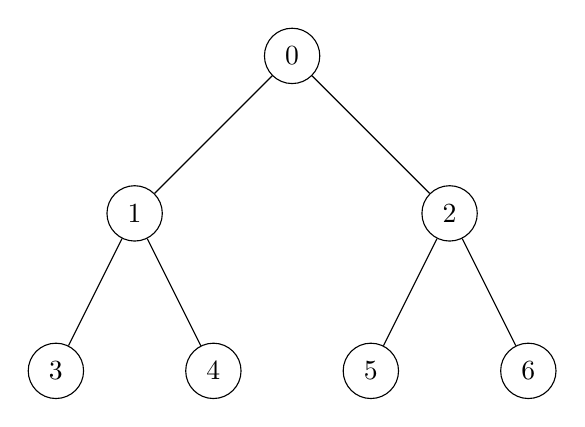
\begin{tikzpicture}
		\tikzset{
			box/.style ={
				circle, %圆形节点
				minimum width =20pt, %最小宽度
				minimum height =20pt, %最小高度
				inner sep=3pt, %文字和边框的距离
				draw=black, %边框颜色
				fill=white
			}
		}
		\node[box] (1) at(0,0){0};
		\node[box] (2) at(-2,-2){1};
		\node[box] (3) at(2,-2){2};
		\node[box] (4) at(-3,-4) {3};
		\node[box] (5) at(-1,-4){4};
		\node[box] (6) at(1,-4){5};
		\node[box] (7) at(3,-4){6};
		\draw[-] (1)--(2);
		\draw[-] (1)--(3);
		\draw[-] (2)--(4);
		\draw[-] (2)--(5);
		\draw[-] (3)--(6);
		\draw[-] (3)--(7);
	\end{tikzpicture}
\end{figure}

\noindent (1) 试写出该Markov链的一步转移概率矩阵 \( \bm{P}_3 \)。\\
(2)对任意顶点 \( i \) (\( 0 \leq i \leq 6 \)),讨论其周期性和常返性。\\
(3)对任意顶点 \( i \) (\( 0 \leq i \leq 6 \)),求质点从 \( i \) 出发后首次返回 \( i \) 所需平均步数 \( \mu_i \)。\\
(4) 在稳态条件下,该Markov链是否时间可逆?需说明理由。\\
(5) 对一般的 \( m \) (\( m \geq 1 \)),试求该Markov链的平稳分布(可不写计算过程)。\\
解:(1)一步转移概率矩阵为
\[
\bm{P}_3=
\begin{pmatrix}
	0 & \frac{1}{2} &\frac{1}{2} & 0 &0 &0&0\\
	\frac{1}{3} & 0&0 & \frac{1}{3} &\frac{1}{3} &0&0\\
	\frac{1}{3} & 0&0 & 0 &0 &\frac{1}{3}&\frac{1}{3}\\
	0 & 1 &0 & 0 &0 &0&0\\
	0 & 1 &0 & 0 &0 &0&0\\
	0 & 0&1 & 0 &0 &0&0\\
	0 & 0&1 & 0 &0 &0&0\\
\end{pmatrix}
\]
(2)所有状态互通,对于每个状态至少需要两步回到自身,则所有的状态的周期为2\\
又Markov链是不可约有限状态的,则所有状态都是正常返的\\
(3)利用有限加权边图上的随机游走的结论,对存在的每条边赋权重$w_{ij}=1$,就满足上述转移概率矩阵,且有\\
\[
\sum\limits_{i,j}^{} w_{ij}=12
\]
上式是因为每条边(共6条)要计数两遍(这样比单独计数每个状态的边之后再相加来的方便)\\
\[
\pi_i=\frac{\sum\limits_{j}^{} w_{ij}}{\sum\limits_{i,j}^{} w_{ij}}
\]
\[
\pi_i=
\begin{cases}
	\frac{1}{6}  &  i=0 \\
	\frac{1}{4} &  i=1,2\\
	\frac{1}{12} & i=3,4,5,6
\end{cases}
\]
\[
\mu_i=\frac{1}{\pi_i}=
\begin{cases}
	6  &  i=0 \\
	4 &  i=1,2\\
	12 & i=3,4,5,6
\end{cases}
\]
(4)当然可逆,这是有限加权边图上的随机游走的结论之一\\
可以代入平稳方程一一验证:\\
\[
\pi_i=\sum\limits_{j}^{} \pi_j P_{ji}
\]
(5)类似(3),仍然对存在的边赋权重$w_{ij}=1$\\
\[
\sum\limits_{i,j}^{} w_{ij}=2(2+\dots+2^{m-1})=2^{m+1}-4
\]
第一层的点连接2个边,最后一层的点连接1个边,其余的点连接3个边,则\\
\[
\pi_i=
\begin{cases}
	\frac{1}{2^m-2}  &  i=0 \\
	\frac{1}{2^{m+1}-4} &  \text{i在第m层}\\
	\frac{3}{2^{m+1}-4} & \text{其他}
\end{cases}
\]\\


\noindent 三、(16分) 设连续时间 Markov 链 $\{X(t), t \geq 0\}$ 的状态空间为 $\{1,2,3\}$,且其 $Q$ 矩阵为
\[
Q = 
\begin{pmatrix}
	-2 & 1 & 1 \\
	0 & -3 & 3 \\
	2 & 0 & -2
\end{pmatrix}
\]
(1) 求对应嵌入链的转移概率矩阵。\\
(2) 当 $t \to \infty$ 时,求 $X(t)$ 的极限分布。\\
解:(1) $Q$ 矩阵指的是对角元为$-v_i$,非对角元为$q_{ij}$的矩阵\\
嵌入链的转移概率矩阵为:
\[
P=
\begin{pmatrix}
	0 & \frac{1}{2} & \frac{1}{2} \\
	0 & 0 & 1 \\
	1 & 0 & 0
\end{pmatrix}
\]
(2)设连续链的极限概率$P_i$,有方程(总离开速率等于总进入速率):\\
$$
\begin{aligned}
	2P_1& =2P_3 \\
	3P_2 & =P_1\\
	2P_3&=P_1+3P_2
\end{aligned}
$$
\[
P_1+P_2+P_3=1
\]
有
\[
P_1=P_3=\frac{3}{7} \quad P_2=\frac{1}{7}
\]
也就是
\[
P(\lim_{t\rightarrow \infty} X(t)=1)=P(\lim_{t\rightarrow \infty} X(t)=3)=\frac{3}{7} \quad P(\lim_{t\rightarrow \infty} X(t)=2)=\frac{1}{7}
\]\\


\noindent 四、(10分) 设 $\{X(t), t \geq 0\}$ 为一个线性生灭过程,且生长率和死亡率分别为 $\lambda_n = n\lambda$ 和 $\mu_n = n\mu$, $n \geq 0$,其中 $\lambda, \mu > 0$ 为给定常数。如果初始状态 $X(0) = 1$,试求灭绝概率 $q= \lim_{t \to \infty} P(X(t) = 0|X(0) = 1)$。\\
解:\\
考虑分支过程,但要注意分支过程是Markov链而非连续链,设此连续链的嵌入链为$\{Y(t), t \geq 0\}$,有转移概率:\\
\[
P_{i,i+1}=\frac{\lambda}{\lambda+\mu} \quad P_{i,i-1}=\frac{\mu}{\lambda+\mu}
\]
同时
\[
\text{从一个个体开始的连续链最终灭绝} \iff \text{从一个个体开始的嵌入链最终灭绝}
\]
因此只需要求嵌入链的灭绝概率即可;注意分支过程的定义为第$t-1$代的每个父代独立产生的第$t$代子代的总数量(相当于父代产生子代之后死亡),而本题父代在产生子代之后还存活,把本题存活的父代看成他自己产生的子代,同时认为父代产生子代之后死亡,记一个父代产生$i$个子代的概率为$P_i$,同时定义:\\
\[
\{\tilde{Y}(t):\tilde{Y}(0)=1\quad \tilde{Y}(t)=Y\left(\sum\limits_{i=0}^{t-1}  \tilde{Y}(i) \right)  \quad t \geq 0\}
\]
则$\{\tilde{Y}(t) \}$为分支过程(相当于分支过程的父代为$Y(t)=n$时,我们认为下一代为$Y(t+n)$)\\
且有:
\[
q= \lim_{t \to \infty} P(Y(t) = 0|Y(0) = 1)= \lim_{t \to \infty} P(\tilde{Y}(t) = 0|\tilde{Y}(0) = 1)
\]
\[
P_0=\frac{\mu}{\lambda+\mu} \quad P_2=\frac{\lambda}{\lambda+\mu}
\]
利用分支过程定理有:
\[
q=P_0+P_2q^2
\]
注意$q$是满足上面方程的最小解:
\[
q=
\begin{cases}
	\frac{\mu}{\lambda}  & \frac{\mu}{\lambda}<1  \\
	1  &  \frac{\mu}{\lambda}\ge 1
\end{cases}
\]
另解:\\
记$q_2=\lim_{t \to \infty} P(X(t) = 0|X(0) = 2)$,对第一次转移取条件\\
\[
q=\frac{\mu}{\lambda+\mu}+\frac{\lambda}{\lambda+\mu}q_2
\]
而从状态2开始的嵌入链如果想灭绝的话,必须先到达1,再从1到达0;在到达1之前可以视1为一个“暂时的”吸收壁,那么可以看到这时从2开始的嵌入链(带有吸收壁1)和从1开始的嵌入链具有相同的性质(它们的转移概率矩阵一样),所以从2“灭绝到”1的概率也是$q$,当到达状态1之后我们认为这个吸收壁被取消了,此时从状态1到达状态0的概率就是$q$,即$q_2=q^2$,得到相同的方程(写到这里也不难发现这其实就是分支过程的方程了)\\

\noindent 五、(14分) 设 $\{B(t), t \geq 0\}$ 为标准 Brown 运动。\\
(1)试求随机变量 $X = B(1) + B(2) + B(3)$ 的分布。\\
(2) 在给定 $B(2) = 1$ 的条件下,试求 $B(1)$ 和 $B(3) + B(4)$ 的联合分布。\\
解:(1)利用独立增量性和平稳增量性:\\
\[
X=3B(1)+2(B(2)-B(1))+(B(3)-B(2))
\]
\[
B(1),B(2)-B(1),B(3)-B(2) \sim N(0,1) \quad \text{且相互独立}
\]
则
\[
X \sim N(0,14)
\]
(2)
\[
B(1)|B(2)=1 \sim N\left(\frac{1}{2},\frac{1}{2}\right)
\]
另一方面$B(3)+B(4)=2B(3)+(B(4)-B(3))$,又
\[
B(3)|B(2)=1 \sim B(2)+(B(3)-B(2))|B(2)=1\sim 1+N(0,1) \sim N(1,1)
\]
\[
B(4)-B(3)|B(2)=1\sim B(4)-B(3)\sim N(0,1)
\]
则
\[
B(3)+B(4)|B(2)=1 \sim N(2,5)
\]
注意Brown运动是Guass过程以及独立增量性($B(1)|B(2)=1$与$B(3)+B(4)|B(2)=1$独立),$(B(1),B(3)+B(4))|B(2)=1$是二元正态分布
\[
(B(1),B(3)+B(4))|B(2)=1 \sim N\left( \left( \frac{1}{2},2\right),
\begin{pmatrix}
	\frac{1}{2} & 0\\
	0& 5
\end{pmatrix}
\right) 
\]
\textbf{RK}:\\
给定$B(t_1)=A,B(t_2)=B$的条件下,对$t_1<s<t_2$,$B(s)$的条件分布为$N\left(A+\frac{(B-A)(s-t_1)}{t_2-t_1},\frac{(s-t_1)(t_2-s)}{t_2-t_1}\right)$\\


\noindent 六、(18分) 考虑一质点在直线上从正整数 $a$ 出发的简单对称随机游走,其中 $0$ 和 $K(K > a)$ 为两个吸收态。设 $S_n$ 表示时刻 $n$ 该质点的位置,$S_0 = a$,而 $T = \min\{n : S_n = 0 \text{ 或 } K\}$,记
\[
M_n = \sum_{k=0}^n S_k - \frac{1}{3} S_n^3
\]
(1) 证明 $\{M_n, n \geq 0\}$ 为鞅。\\
(2) 试利用停时定理来求解 $\mathbb{E}[\sum_{k=0}^TS_k]$。\\
解:(1)利用$\mathbb{E}[X|U]=\mathbb{E}[\mathbb{E}[X|U,V]|U]$,并注意$S_1,\dots,S_n$实际上包含了$M_1,\dots,M_n$的所有信息\\
$$
\begin{aligned}
	\mathbb{E}[M_{n+1}|M_1,...,M_n] &= \mathbb{E}[\mathbb{E}[M_{n+1}|S_1,...,S_n]|M_1,...,M_n] \\
\end{aligned}
$$
其中
$$
\begin{aligned}
	\mathbb{E}[M_{n+1}|S_1,...,S_n] & =\mathbb{E}\left[\sum\limits_{k=0}^{n} S_k +S_{n+1}-\frac{1}{3}\left( S_n+X_{n+1}\right) |S_1,...,S_n\right] \\
	&=\mathbb{E}\left[\sum\limits_{k=0}^{n} S_k +S_{n}+X_{n+1}-\frac{1}{3}\left( S_n+X_{n+1}\right)|S_1,...,S_n \right]\\
	& \stackrel{X_{n+1}\text{与}S_1,...,S_n\text{独立}}=\sum\limits_{k=0}^{n} S_k+S_n+\mathbb{E}[X_{n+1}]-\frac{1}{3}S_n^3-\frac{1}{3}\mathbb{E}[X_{n+1}^3]-S_n^2\mathbb{E}[X_{n+1}]-\mathbb{E}[X_{n+1}^2]S_n\\
	&=\sum_{k=0}^n S_k - \frac{1}{3} S_n^3\\
	&=M_n
\end{aligned}
$$
这就说明了
\[
\mathbb{E}[M_{n+1}|M_1,...,M_n]=\mathbb{E}[\mathbb{E}[M_{n+1}|S_1,...,S_n]|M_1,...,M_n]=\mathbb{E}[M_n|M_1,...,M_n]=M_n
\]
另外
\[
\mathbb{E}[|M_n|]\le \mathbb{E}\left[\sum_{k=0}^n S_k  \right] +\frac{1}{3}\mathbb{E}[S_n^3] < \infty
\]
即$\{M_n, n \geq 0\}$ 为鞅\\
(2)先验证一下鞅停止定理的条件
$$
\begin{aligned}
	\mathbb{E}[|M_{n+1}-M_n|\mid M_1,...,M_n] & =\mathbb{E}\left[|S_{n+1}-\frac{1}{3}(S_{n+1}^3-S_n^3)|\mid M_1,...,M_n\right] \\
	&   =\mathbb{E}\left[|S_{n+1}-\frac{1}{3}(X_{n+1}^3+3S_n^2X_{n+1}+3S_nX_{n+1}^2)|\mid M_1,...,M_n\right] \\
	&\stackrel{\text{三角不等式}}<M
\end{aligned}
$$
则$$\mathbb{E}[M_T]=\mathbb{E}\left[ \sum_{k=0}^T S_k - \frac{1}{3} S_T^3\right] =\mathbb{E}[M_0]=a-\frac{1}{3}a^3$$\\
由赌徒破产模型(开始财富为$a$,公平赌模型下,财富先到达$K$而不是0的概率):
\[
P(S_T=K)=\frac{a}{K}
\]
\[
\mathbb{E}\left[S_T^3 \right] =P(S_T=K)K^3=aK^2
\]
最后
\[
\mathbb{E}\left[ \sum_{k=0}^TS_k\right] =\frac{1}{3}aK^2+a-\frac{1}{3}a^3
\]\\


\noindent 七、(附加题, 10分) 证明标准 Brown 运动 $\{B(t), t \geq 0\}$ 在任一区间 $[0,t]$ 上的二次变差为 $t$,即对区间 $[0,t]$ 上的任意分割 $0 = t_0 < t_1 < \cdots < t_n < t_{n+1} = t$,当 $n \to \infty$ 时,若最大间隔 $\max_{0 \leq i \leq n}(t_{i+1} - t_i) \to 0$,则有 $Q_n = \sum_{k=0}^n [B(t_{k+1}) - B(t_k)]^2$ 依概率收敛到 $t$。\\
解:证明依概率收敛$P(|Q_n-t|\ge \epsilon)\rightarrow0$考虑Markov不等式或者Chebyshev不等式\\
$$
\begin{aligned}
	\mathbb{E}[Q_n] & =\mathbb{E}\left[\sum_{k=0}^n [B(t_{k+1}) - B(t_k)]^2 \right]  \\
	& =\sum_{k=0}^n \mathbb{E}\left[ [B(t_{k+1}) - B(t_k)]^2\right] 
\end{aligned}
$$
另外
\[
B(t_{k+1})-B(t_k) \sim N(0,t_{k+1}-t_k) \quad \mathbb{E}\left[ [B(t_{k+1}) - B(t_k)]^2\right] =t_{k+1}-t_k
\]
则
\[
\mathbb{E}[Q_n]=\sum_{k=0}^n \mathbb{E}\left[ [B(t_{k+1}) - B(t_k)]^2\right] =t
\]
由独立增量性:
$$
\begin{aligned}
	\operatorname{Var}(Q_n) & =\operatorname{Var}\left(\sum_{k=0}^n [B(t_{k+1}) - B(t_k)]^2 \right)  \\
	& =\sum_{k=0}^n \operatorname{Var}\left( [B(t_{k+1}) - B(t_k)]^2\right)
\end{aligned}
$$
记$N_k=B(t_{k+1})-B(t_k) \sim N(0,t_{k+1}-t_k)$\\
$$
\begin{aligned}
	\operatorname{Var}(N_k)&=\mathbb{E}[N_k^4]-\left(\mathbb{E}[N_k^2] \right)^2\\
	& =3(t_{k+1}-t_k)^2-(t_{k+1}-t_k)^2\\
	& =2(t_{k+1}-t_k)^2
\end{aligned}
$$
利用Chebyshev不等式\\
$$
\begin{aligned}
	P(|Q_n-t|\ge \epsilon)&\le \frac{\operatorname{Var}(Q_n)}{\epsilon^2}\\
	&\le \frac{2\sum_{k=0}^n(t_{k+1}-t_k)^2}{\epsilon^2}\\
	&\le \frac{2\left( \sum_{k=0}^n(t_{k+1}-t_k)\right)\max\{
		t_{k+1}-t_k\}}{\epsilon^2}\\
	&\le \frac{2t\max\{
		t_{k+1}-t_k\}}{\epsilon^2}\\
	&\rightarrow 0
\end{aligned}
$$
这就说明了依概率收敛\\
\textbf{RK}:\\
对正态分布的高阶矩有
$$
\begin{aligned}
	X &\sim N(0,1)\\
	\forall k=2m>0&\quad \mathbb{E}[X^k]=(2m-1)!!
\end{aligned}
$$
也可以通过$N(\mu,\sigma^2)$的矩母函数$$M(t)=e^{\mu t+\frac{1}{2}\sigma^2t^2}$$或者特征函数$$\phi(t)=e^{i\mu t+\frac{1}{2}\sigma^2t^2}$$来获得高阶矩的信息\\
\newpage
\section{\centering 24实用随机过程期末}
\noindent 1.(每小题 6 分,总 30 分)设有一个质点在如图所示的二叉树上(共 $m=3$ 层)作随机游走:它从顶点 0 出发,每隔单位时间等概率沿边转移到某一个邻点上.以 $X_{n}$ 表示该质点经过 $n$ 步跳之后所在顶点的编号,则 $\left\{X_{n}, n \geq 0\right\}$ 为一个 Markov 链。\\
\begin{figure}[h!]
	\centering
	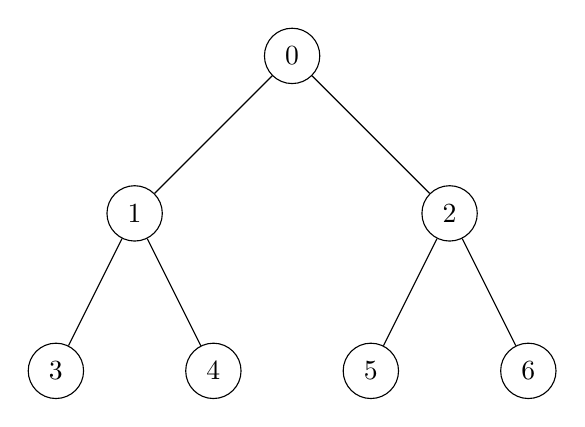
\begin{tikzpicture}
		\tikzset{
			box/.style ={
				circle, %圆形节点
				minimum width =20pt, %最小宽度
				minimum height =20pt, %最小高度
				inner sep=3pt, %文字和边框的距离
				draw=black, %边框颜色
				fill=white
			}
		}
		\node[box] (1) at(0,0){0};
		\node[box] (2) at(-2,-2){1};
		\node[box] (3) at(2,-2){2};
		\node[box] (4) at(-3,-4) {3};
		\node[box] (5) at(-1,-4){4};
		\node[box] (6) at(1,-4){5};
		\node[box] (7) at(3,-4){6};
		\draw[-] (1)--(2);
		\draw[-] (1)--(3);
		\draw[-] (2)--(4);
		\draw[-] (2)--(5);
		\draw[-] (3)--(6);
		\draw[-] (3)--(7);
	\end{tikzpicture}
\end{figure}

\noindent (1)试写出 $\left\{X_{n}, n \geq 0\right\}$ 的一步转移概率矩阵 $\bm{P}_3$ .\\
(2)对任意顶点 $k(0 \leq k \leq 6)$ ,讨论其周期性和常返性.\\
(3)对任意顶点 $k(0 \leq k \leq 6)$ ,求质点从 $k$ 出发后第一次返回到 $k$ 所需平均步数 $\mu_{k}$ .\\
(4)在稳态条件下,该 Markov 链是否都是时间可逆的?证明你的结论.\\
(5)对一般的 $m(m \geq 1)$ ,试求该 Markov 链的平稳分布.\\
解:(1)一步转移概率矩阵为
\[
\bm{P}_3=
\begin{pmatrix}
	0 & \frac{1}{2} &\frac{1}{2} & 0 &0 &0&0\\
	\frac{1}{3} & 0&0 & \frac{1}{3} &\frac{1}{3} &0&0\\
	\frac{1}{3} & 0&0 & 0 &0 &\frac{1}{3}&\frac{1}{3}\\
	0 & 1 &0 & 0 &0 &0&0\\
	0 & 1 &0 & 0 &0 &0&0\\
	0 & 0&1 & 0 &0 &0&0\\
	0 & 0&1 & 0 &0 &0&0\\
\end{pmatrix}
\]
(2)所有状态互通,对于每个状态至少需要两步回到自身,则所有的状态的周期为2\\
又Markov链是不可约有限状态的,则所有状态都是正常返的\\
(3)利用有限加权边图上的随机游走的结论,对存在的每条边赋权重$w_{ij}=1$,就满足上述转移概率矩阵,且有\\
\[
\sum\limits_{i,j}^{} w_{ij}=12
\]
上式是因为每条边(共6条)要计数两遍(这样比单独计数每个状态的边之后再相加来的方便)\\
\[
\pi_i=\frac{\sum\limits_{j}^{} w_{ij}}{\sum\limits_{i,j}^{} w_{ij}}
\]
\[
\pi_i=
\begin{cases}
	\frac{1}{6}  &  i=0 \\
	\frac{1}{4} &  i=1,2\\
	\frac{1}{12} & i=3,4,5,6
\end{cases}
\]
\[
\mu_i=\frac{1}{\pi_i}=
\begin{cases}
	6  &  i=0 \\
	4 &  i=1,2\\
	12 & i=3,4,5,6
\end{cases}
\]
(4)当然可逆,这是有限加权边图上的随机游走的结论之一\\
可以代入平稳方程一一验证:\\
\[
\pi_i=\sum\limits_{j}^{} \pi_j P_{ji}
\]
(5)类似(3),仍然对存在的边赋权重$w_{ij}=1$\\
\[
\sum\limits_{i,j}^{} w_{ij}=2(2+\dots+2^{m-1})=2^{m+1}-4
\]
第一层的点连接2个边,最后一层的点连接1个边,其余的点连接3个边,则\\
\[
\pi_i=
\begin{cases}
	\frac{1}{2^m-2}  &  i=0 \\
	\frac{1}{2^{m+1}-4} &  \text{i在第m层}\\
	\frac{3}{2^{m+1}-4} & \text{其他}
\end{cases}
\]\\


\noindent 2.(每小题 7 分,总 21 分)考察一个出租车的车站,出租车与顾客分别按速率为每分钟 1 辆和每分钟 2 人的 Poisson 过程到达.无论有多少辆出租车在那里,新来的出租车都会等待;然而,若顾客到来发现没有出租车就会离去.\\
(1)求在等待的出租车的平均数;\\
(2)问到达的顾客中有多少比例的人能搭到出租车?\\
(3)求该出租车的车站从出现没有出租车在等待的时刻开始到再次出现没有出租车在等待时的期望间隔时间。\\
解:构建一个连续时间马氏链 $X(t)$ 表示在 $t$ 时刻出租车数,则 $X(t) \in \mathbb{N}$ ,该马氏链可视为生灭过程,列出其增长率 $\lambda_i=1(i \geq 0)$ ,其死亡率为 $\mu_i=2(i \geq 1)$ 。首先求解其平稳分布 $P_i$ ,求解方程\\
$$
\begin{aligned}
	\lambda_0 P_0 & =\mu_1 P_1 \\
	\lambda_1 P_1+\mu_1 P_1 & =\mu_2 P_2+\lambda_0 P_0 \\
	\lambda_2 P_2+\mu_2 P_2 & =\mu_3 P_3+\lambda_1 P_1 \\
	& \ldots
\end{aligned}
$$
可以解出平稳概率为 $P_i=2^{-i-1}(i \geq 0)$ 。\\
(1)平均数为
$$
\sum_{i=1}^{\infty} i P_i=\sum_{i=1}^{\infty} \frac{i}{2^{i+1}}=1
$$
(2)比例为 $1-P_0=\frac{1}{2}$ 。\\
(3)把没有出租车开始视为一次更新,则没有出租车与有出租车构成交替更新过程,从而
$$
P_0=\frac{\mathbb{E}[\text { 没有出租车持续的时间 }]}{\mathbb{E}[\text { 没有出租车持续的时间 }]+\mathbb{E}[\text { 有出租车持续的时间 }]},
$$
由于 $\mathbb{E}[$ 没有出租车持续的时间 $]=\frac{1}{\lambda_0}=1$ ,于是可知 $\mathbb{E}[$ 没有出租车持续的时间 $]+\mathbb{E}[$ 有出租车持续的时间 $]=$ 2。\\
\textbf{RK}:\\
对于$M/ M / 1$排队系统$(\lambda_i=\lambda(i \geq 0)\quad \mu_i=\mu(i \geq 1))$,利用生灭过程的极限概率:
\[
P_0=\left[1+\sum\limits_{n=1}^{\infty} \frac{\lambda_0 \dots \lambda_{n-1}}{\mu_1 \dots \mu_n} \right] ^{-1}
\]
\[
P_n=\frac{\lambda_0 \dots \lambda_{n-1}}{\mu_1 \dots \mu_n\left(1+\sum\limits_{n=1}^{\infty} \frac{\lambda_0 \dots \lambda_{n-1}}{\mu_1 \dots \mu_n} \right) }
\]
设$\rho=\frac{\lambda}{\mu}$,则平稳概率为:
\[
\pi_n=(1-\rho)\rho^n
\]
在等待的总人数为:
\[
L=\sum\limits_{n=0}^{\infty} nP_n=\frac{\rho}{1-\rho}
\]
又两次回到状态0的平均时间$$\mu_{00}=\frac{1}{v_0P_0}=\frac{1}{\lambda(1-\rho)}$$\\
则关于忙期$B$有:
\[
\mathbb{E}[B]=\mu_{00}-\frac{1}{\lambda}=\frac{1}{\mu-\lambda}
\]\\
这是22期末第三题下的\textbf{RK}的直接推论\\


\noindent 3.(每小题 6 分,总 12 分)考虑一个连续时间的生灭过程 $\{X(t), t \geq 0\}$ ,出生率为 $\left\{\lambda_{i}, i \geq 0\right\}$ ,死亡率为 $\left\{\mu_{j}, j \geq 1\right\}$ 。对给定的 $k>0$ ,当系统处于状态 $k$ ,等待进入状态 $k+1$ 的等待时间记为 $T_{k, k+1}$ ;当系统处于状态 $k$ ,等待进入状态 $k-1$ 的等待时间记为 $T_{k, k-1}$ .\\
(1)问 $T_{k, k+1}$ 和 $T_{k, k-1}$ 分别服从什么分布?\\
(2)问 $T_{k, k+1}$ 和 $T_{k, k-1}$ 是否相互独立?\\
解:(1)注意已经给定下一次转移的状态了,则:
\[
T_{k,k+1} \sim \mathrm{Exp}(\lambda_i) \quad T_{k,k-1} \sim \mathrm{Exp}(\mu_i)
\]
(2)独立,这是连续$Markov$链的定义\\


\noindent 4.(第 1 小题 7 分,第 2 小题 12 分,总 19 分).设 $\{B(t), t \geq 0\}$ 为标准 Brown 运动.\\
(1)对于人员 $0<s<t$ ,证明 $B(s)-\frac{s}{t} B(t)$ 与 $B(t)$ 相互独立.\\
(2)给定 $B(1)=0, B(3)=u \in \mathbb{R}$ ,求事件 $\{B(2)>u, B(4)>u\}$ 发生的概率.\\
解:(1)\\
Brown运动为Gauss过程,则$\left(B(s)-\frac{s}{t} B(t), B(t)\right) $为二元正态分布,由多元正态分布的性质只需要证明$\operatorname{Cov}\left(B(s)-\frac{s}{t} B(t), B(t)\right)=0 $即可
$$
\begin{aligned}
	\operatorname{Cov}\left(B(s)-\frac{s}{t} B(t), B(t)\right) & =\operatorname{Cov}\left(B(s),B(t) \right)-\frac{s}{t}\operatorname{Var}\left(B(t) \right)  \\
	& =s-\frac{s}{t}t\\
	&=0
\end{aligned}
$$
这就说明了独立性\\
(2)\\
给定$B(t_1)=A,B(t_2)=B$的条件下,对$t_1<s<t_2$,$B(s)$的条件分布为$N\left(A+\frac{(B-A)(s-t_1)}{t_2-t_1},\frac{(s-t_1)(t_2-s)}{t_2-t_1}\right)$\\
则
\[
B(2)|B(1)=0,B(3)=u \sim N\left(\frac{u}{2},\frac{1}{2} \right) 
\]
\[
B(4)|B(1)=0,B(3)=u \sim B(3)+\left( B(4)-B(3)\right)|B(1)=0,B(3)=u \sim u+N(0,1) \sim N(u,1) 
\]
则由独立增量性:
$$
\begin{aligned}
	P\left(B(2)>u, B(4)>u|B(1)=0,B(3)=u \right)  & = P\left(B(2)>u |B(1)=0,B(3)=u \right)P\left(B(4)>u|B(1)=0,B(3)=u \right)\\
	& =P\left( \frac{\left( N\left(\frac{u}{2},\frac{1}{2}\right) -\frac{u}{2}\right)}{\sqrt{\frac{1}{2}}} > \frac {u-\frac{u}{2}}{\sqrt{\frac{1}{2}}}\right) P\left(N(u,1) -u>u-u \right) \\
	&=P\left( N(0,1)>\frac{\sqrt{
			2}u}{2}\right)\cdot \frac{1}{2}\\
	&=\frac{1}{2}\left(1-\Phi\left(\frac{\sqrt{
			2}u}{2} \right)  \right)  
\end{aligned}
$$\\
其中$\Phi(x)$为$N(0,1)$的分布函数\\


\noindent 5.(每小题 6 分,总 18 分)设 $\left\{Y_{n}, n \geq 1\right\}$ 为独立同分布的随机变量序列,$f_{0}$ 和 $f_{1}$ 是两个概率密度函数,且满足对任意 $x \in \mathbb{R}$ ,有 $f_{0}(x)>0, f_{1}(x)>0$ .定义

$$
X_{n}=\prod_{i=1}^{n} \frac{f_{1}\left(Y_{i}\right)}{f_{0}\left(Y_{i}\right)}
$$

\noindent (1)证明:如果 $f_{0}$ 为 $Y_{1}$ 的概率密度函数,则 $\left\{X_{n}, n \geq 1\right\}$ 为一个鞅序列.\\
(2)证明:如果 $f_{1}$ 为 $Y_{1}$ 的概率密度函数,则 $\left\{X_{n}, n \geq 1\right\}$ 为一个下鞅序列.\\
(3)证明:如果 $f_{0}$ 为 $Y_{1}$ 的概率密度函数,则对任意 $a>0$ ,

$$
\mathrm{P}\left(\max \left\{X_{1}, X_{2}, \ldots, X_{n}\right\} \right) \leq \frac{1}{a}, \quad n>1 .
$$
解:(1)\\
$$
\begin{aligned}
	\mathbb{E}[X_{n+1}|X_1,...,X_n]&=X_n\mathbb{E}\left[ \frac{f_1(Y_{n+1})}{f_0(Y_{n+1})}|X_1,...,X_n\right] \\
	&=X_n \int_{\mathbb{R}} \frac{f_1(x)}{f_0(x)} f_0(x) dx\\
	&=X_n \int_{\mathbb{R}}f_1(x) dx\\
	&=X_n
\end{aligned}
$$
另外注意$X_n$非负
\[
\mathbb{E}[|X_n|]=\mathbb{E}[X_n]=\mathbb{E}[X_1]=1<\infty
\]
则 $\left\{X_{n}, n \geq 1\right\}$ 为鞅\\
(2)\\
$$
\begin{aligned}
	\mathbb{E}[X_{n+1}|X_1,...,X_n]&=X_n\mathbb{E}\left[ \frac{f_1(Y_{n+1})}{f_0(Y_{n+1})}|X_1,...,X_n\right] \\
	&=X_n \int_{\mathbb{R}} \frac{f_1(x)}{f_0(x)} f_1(x) dx\\
\end{aligned}
$$
利用Cauthy-Schwarz积分不等式
\[
\left(\int fg \right)^2 \le \int f^2 \int g^2 
\]
可以得到
\[
\left(\int_{\mathbb{R}} f_1(x)dx \right)^2 \le \left(\int_{\mathbb{R}} f_0(x)dx \right)\left(\int_{\mathbb{R}} \frac{f_1^2(x)}{f_0(x)}dx \right)   
\]
注意到密度的积分为1,即:
$$\int_{\mathbb{R}} f_1(x)dx=\int_{\mathbb{R}} f_0(x)dx=1$$
则
\[
\int_{\mathbb{R}} \frac{f_1^2(x)}{f_0(x)}dx \ge 1
\]
\[
\mathbb{E}\left[ \frac{f_1(Y_{n+1})}{f_0(Y_{n+1})}|X_1,...,X_n\right] \ge 1
\]
另外
\[
\mathbb{E}[|X_n|]<\infty
\]
则$\left\{X_{n}, n \geq 1\right\}$ 为下鞅\\
(3)\\
$X_n$恒正,由下鞅的Kolmogorov不等式就有\\
\[
P(\max\{X_1,...,X_n\}>a) \le \frac{\mathbb{E}[X_n]}{a}=\frac{\mathbb{E}[X_1]}{a}=\frac{1}{a}
\]\\
\newpage
\section{\centering 22实用随机过程期末}
\noindent 1.(每小题 3 分,总 18 分)判断题\\
(1)一个时间可逆的连续时间马氏链的嵌入链也是时间可逆的\\
答案:正确\\
但是嵌入链可逆不一定可以推出连续Markov链可逆\\


\noindent (2)设 $i \leftrightarrow j, j$ 的周期为 $d>1$ ,则 $\lim _{n \rightarrow \infty} P_{i j}^{n d}=d / \mu_{j j}$ ,其中 $\mu_{j j}$ 是马氏链相邻两次访问状态 $j$ 的期望间隔时间\\
答案:错误\\
反例:考虑一个连续Markov链,其只有两个状态${1,2}$,且状态$1$只能转移到$2$,$2$只能转移到$1$,则这两个状态的周期为$2$,但是$\lim_{n \rightarrow \infty}P_{12}^{n d}=0$\\
成立的结论应该是: $j$ 的周期为 $d>1$ ,则 $\lim _{n \rightarrow \infty} P_{j j}^{n d}=d / \mu_{j j}$ ,其中 $\mu_{j j}$ 是马氏链相邻两次访问状态 $j$ 的期望间隔时间\\


\noindent (3)设 $S$ 和 $T$ 是一个随机变量序列的停时,则 $\min \{S, T\}$ 也是一个停时\\
答案:正确\\
$S,T$均由随机变量序列$Z_1,...,Z_n$决定且$P(S<\infty)=1 \quad P(T<\infty)=1$\\
那么$\min \{S,T\}$由$Z_1,...,Z_n$决定且$P(\min \{S,T\}<\infty)=1$,这就说明其为停时\\


\noindent (4)半马氏过程是一类特殊的连续时间马氏过程\\
答案:错误\\
连续时间马氏过程是一类特殊的半马氏过程\\


\noindent (5)设 $\left\{Z_{n}, n \geq 1\right\}$ 为二阶矩存在有限的鞅,定义 $X_{k}=Z_{k}-Z_{k-1}, k \geq 1$ ,且约定 $Z_{0}=0$ ,则 $\operatorname{Var}\left(Z_{n}\right)=\sum_{k=1}^{n} \operatorname{Var}\left(X_{k}\right)$ \\
答案:正确\\
这道题是书上习题6.2\\
\[
\operatorname{Var}\left(Z_n \right)=\operatorname{Var}(\sum_{i=1}^{n} X_i)=\sum_{i=1}^{n} \operatorname{Var}(X_i)+2\sum\limits_{1 \le i <j \le n }^{} \operatorname{Cov}(X_i,X_j) 
\]
所以只需要证明$\sum\limits_{1 \le i <j \le n }^{} \operatorname{Cov}(X_i,X_j)=0 $即可\\
先证明一个引理:$\mathbb{E}\left[Z_n \mid Z_1, \ldots, Z_k\right] =Z_k$\\
$$
\begin{aligned}
	\mathbb{E}\left[Z_n \mid Z_1, \ldots, Z_k\right] & =\mathbb{E}\left[\mathbb{E}\left[Z_n \mid Z_1, \ldots, Z_{n-1}\right] \mid Z_1, \ldots, Z_k\right] \\
	& =\mathbb{E}\left[Z_{n-1} \mid Z_1, \ldots, Z_k\right] \\
	& =\mathbb{E}\left[Z_t \mid Z_1, \ldots, Z_k\right] \\
	& =Z_k
\end{aligned}
$$
这里用到了双重条件期望公式:$\mathbb{E}[X|U]=\mathbb{E}[\mathbb{E}[X|U,V]|U]$\\
即证对$\forall i<j, \operatorname{Cov}\left(X_i, X_j\right)=0 $事实上,由引理知\\
$$
\begin{aligned}
	&\begin{aligned}
		\mathbb{E}\left[X_i\right] & =\mathbb{E}\left[Z_i\right]-\mathbb{E}\left[Z_{i-1}\right]=0, \\
		\operatorname{Cov}\left(X_i, X_j\right) & =\mathbb{E}\left[X_i X_j\right] \\
		& =\mathbb{E}\left[\left(Z_i-Z_{i-1}\right)\left(Z_j-Z_{j-1}\right)\right] \\
		& =\mathbb{E}\left[\mathbb{E}\left[\left(Z_i-Z_{i-1}\right)\left(Z_j-Z_{j-1}\right) \mid Z_1, \ldots, Z_i\right]\right] \\
		& =\mathbb{E}\left[\left(Z_i-Z_{i-1}\right) \mathbb{E}\left[\left(Z_j-Z_{j-1}\right) \mid Z_1, \ldots, Z_i\right]\right] \\
		& =\mathbb{E}\left[\left(Z_i-Z_{i-1}\right)\left(Z_i-Z_i\right)\right] \\
		& =0
	\end{aligned}
\end{aligned}
$$\\


\noindent (6)在布朗运动中,从 0 状态到达其它任一状态的平均时间皆为正无穷\\
答案:正确\\
从0状态到达其他任意状态的平均时间为正无穷,但是到达其他状态的概率是1\\


\noindent 2.(总 21 分,其中附加题 5 分)现有一个粒子在一个圆周上做随机游动,圆周上有 12个状态,按顺时针方向分别编号为 $1,2, \ldots, 12$ 。设 $X_{n}$ 表示粒子在时刻 $n$(即第 $n$ 步跳以后)所处的状态,且假设粒子的每一步跳都会等概率地往顺时针或逆时针方向跳一步.\\
(1)(8 分)该过程长时间运行下去,求粒子处在状态 $k$ 的概率;\\
(2)(8 分)求粒子从状态 12 出发重新回到 12 状态平均需要跳的步数;\\
(3)【附加题, 5 分】粒子从状态 12 出发,再次回到状态 12 之前访问过其它所有的 11 个状态的概率有多大?\\
解:\\
(1)转移概率矩阵为:\\
\[
\begin{pmatrix}
	0 & \frac{1}{2} & 0      & \cdots & \frac{1}{2} \\
	\frac{1}{2} & 0 & \frac{1}{2} & \cdots & 0 \\
	0      & \ddots & \ddots & \ddots & \vdots \\
	\vdots & \cdots & \frac{1}{2}& 0 & \frac{1}{2}\\
	\frac{1}{2}      & \cdots & 0      & \frac{1}{2}& 0
\end{pmatrix}
\]
这是一个双随机Markov链(见\textbf{RK})\\
因此$\forall i \quad \pi_i=\frac{1}{12}$\\
(2)$\mu_{12,12}=\frac{1}{\pi_{12}}=12$\\
(3)对第一次转移的状态取条件\\
\[
P(\text{从状态 12 出发,再次回到状态 12 之前访问过其它所有的 11 个状态}) 
\]
\[
= \frac{1}{2}P(\text{回到12前访问所有其他状态} \mid \text{第一步转移到1}) 
\]
\[
+ \frac{1}{2}P(\text{回到12前访问所有其他状态} \mid \text{第一步转移到11})
\]
由于转移概率均为$\frac{1}{2}$,计算$P(\text{回到12前访问所有其他状态} \mid \text{第一步转移到1})$即可\\
由赌徒破产模型,这就相当于从财富1开始,赌徒先赢到11而不输光的概率,即$\frac{1}{11}$\\
则
\[
P(\text{从状态 12 出发,再次回到状态 12 之前访问过其它所有的 11 个状态}) =\frac{1}{11}
\]
\textbf{RK}:双随机Markov链指的是转移概率矩阵的每一列的和为1的Markov链\\
有$M$个状态$1,2,...,M$的Markov链有平稳概率:$\forall i,\pi_i=\frac{1}{M}$\\
这可以通过直接代入平稳方程:$\pi_i=\sum\limits_{j}^{}\pi_j P_{ji}$来得到\\


\noindent 3.(每小题 6 分,总 24 分)假设一个加油站有 3 个加油停车位和 2 个加油工,来到加油站的汽车按一个 Poisson 过程到达,平均每 10 分钟到达一辆.如果驾驶员发现加油车位已经被占用,则自行离开.假设每辆车加油所需时间服从均值为 20 分钟的指数分布.\\
(1)求到达加油站没有加油直接离开的车辆的平均占比;\\
(2)求稳态情形下在加油站等待或正在加油的平均车辆个数;\\
(3)求稳态情形下相邻两个忙期开始的平均间隔时间;\\
(4)求稳态情形下一个忙期之内平均加油的车辆数\\
解:构建一个连续时间马氏链 $X(t)$ 表示在 $t$ 时刻加油站停靠车辆数,则 $X(t) \in\{0,1,2,3\}$ ,该马氏链可视为生灭过程,列出其增长率 $\lambda_0=\lambda_1=\lambda_2=\frac{1}{10}$ ,其死亡率为 $\mu_1=\frac{1}{20}, \mu_2=\mu_3=\frac{1}{10}$ 。首先求解其平稳分布 $P_i$ ,求解方程\\
$$
\begin{aligned}
	\lambda_0 P_0 & =\mu_1 P_1 \\
	\lambda_1 P_1+\mu_1 P_1 & =\mu_2 P_2+\lambda_0 P_0 \\
	\lambda_2 P_2+\mu_2 P_2 & =\mu_3 P_3+\lambda_1 P_1 \\
	\lambda_2 P_2 & =\mu_3 P_3 .
\end{aligned}
$$
可以解出平稳概率为 $P_0=\frac{1}{7}, P_1=P_2=P_3=\frac{2}{7}$ 。\\
(1)即求解加油站有三辆车的时间的平均占比,长程状态下该事件占比即为 $P_3$ 。\\
(2)平均车辆数为 $P_1+2 P_2+3 P_3=\frac{12}{7}$ 。\\
(3)当加油站内没有汽车时为闲期,当加油站内有汽车时为忙期。稳态下两个忙期开始的时间间隔即为一个忙期加一个闲期的平均时间,该时间也会和两个闲期开始的时间间隔一致,把闲期开始当做一次更新,因此一个更新区间内包含一个闲期和一个忙期,可视作交替更新过程,在稳态情况下可视作更新过程已运作无穷长时间,因此\\
$$
P_0=\frac{\mathbb{E}[\text { 一个闲期的长度 }]}{\mathbb{E}[\text { 一个闲期的长度 }]+\mathbb{E}[\text { 一个忙期的长度 }]} .
$$
由于闲期长度期望是已知的为 10 ,于是所求$\mathbb{E}[$ 一个闲期的长度 $]+\mathbb{E}[$ 一个忙期的长度 $]=70$ .\\
另一种方法:由于一个忙期开始时油站内汽车数必然为 1 ,因此忙期持续时间为油站内汽车数量为 1 时第一次返回汽车数量为 0 时所需时间,设油站内汽车数为 $i$ 时第一次到汽车数为 0 时所需时间为 $T_i$ ,则由全概率公式\\
$$
\begin{aligned}
	& \mathbb{E} [T_1]=\frac{1}{3} \frac{1}{\lambda_1+\mu_1}+\frac{2}{3}\left(\mathbb{E} [T_2]+\frac{1}{\lambda_1+\mu_1}\right) \\
	& \mathbb{E} [T_2]=\frac{1}{2}\left(\frac{1}{\lambda_2+\mu_2}+\mathbb{E} [T_1]\right)+\frac{1}{2}\left(\frac{1}{\lambda_2+\mu_2}+\mathbb{E} [T_3]\right) \\
	& \mathbb{E} [T_3]=\frac{1}{\mu_3}+\mathbb{E} [T_2]
\end{aligned}
$$
解得 $\mathbb{E} [T_1]=60$ ,这表明忙期平均时间为 60 ,从而
$$\mathbb{E}[ \text{一个闲期的长度} ]+\mathbb{E}[ \text{一个忙期的长度} ]=70$$
(4)同上,将进入闲期当做一次更新,把加油车辆数看做报酬,于是由更新报酬过程知\\
$$
\lim _{t \rightarrow \infty} \frac{\mathbb{E}[\text { 在 }(0, t) \text { 加油车辆总数 }]}{t}=\frac{\mathbb{E}[\text { 一个忙期内加油车辆总数 }]}{\mathbb{E}[\text { 一个闲期的长度 }]+\mathbb{E}[\text { 一个忙期的长度 }]} .
$$
另一方面,在稳态情况下\\
\[
\lim _{t \rightarrow \infty} \frac{\mathbb{E}[\text { 在 }(0, t) \text { 加油车辆总数 }]}{t}=\text { 实际进入加油车辆比例 } \times \text { 车辆到来速率 }
\]
\[
=\frac{5}{7} \times \frac{1}{10}=\frac{1}{14} \text {. }
\]
于是可得一个忙期内平均加油车辆数为 5 .\\
\textbf{RK}:(1)对于连续Markov链,利用交替更新过程,把回到$i$记录为一次更新,停留在$i$记为系统在“开”状态,则两次回到状态$i$的平均时间与极限概率有关系:$\mu_{ii}=\frac{1}{v_i P_i}$,其中$v_i$是离开状态$i$的总速率\\
(2)对于$M/ M/ s$排队系统,顾客Poisson到达的速率为$\lambda$,每条服务链服务的速率为$\mu$,利用生灭过程的极限概率:\\
\[
P_0=\left[1+\sum\limits_{n=1}^{\infty} \frac{\lambda_0 \dots \lambda_{n-1}}{\mu_1 \dots \mu_n} \right] ^{-1}
\]
\[
P_n=\frac{\lambda_0 \dots \lambda_{n-1}}{\mu_1 \dots \mu_n\left(1+\sum\limits_{n=1}^{\infty} \frac{\lambda_0 \dots \lambda_{n-1}}{\mu_1 \dots \mu_n} \right) }
\]
并记流量强度$\rho=\frac{\lambda}{s\mu}$\\
则极限概率为:
\[
P_0=\left[1+\sum\limits_{n=1}^{s} \frac{1}{n!} \left( \frac{\lambda}{\mu}\right) ^n+\frac{1}{s!} \frac{\rho}{1-\rho} \left(\frac{\lambda}{\mu} \right) ^s \right] ^{-1}
\]
\[
P_n=
\begin{cases}
	\frac{1}{n!} \left(\frac{\lambda}{\mu} \right)^n P_0  &  n \le s \\
	\rho^{n-s} \frac{1}{s!} \left(\frac{\lambda}{\mu} \right)^s P_0  &  n>s
\end{cases}
\]
系统内平均总顾客数:
\[
L=\sum\limits_{n=0}^{\infty} nP_n=\frac{\lambda}{\mu}+\frac{1}{s!} \left(\frac{\lambda}{\mu} \right)^s \frac{\rho}{\left(1-\rho \right)^2 } P_0
\]
忙期的期望利用(1)有:
\[
E[B]=\frac{1}{v_0P_0}-\frac{1}{\lambda}=\frac{1}{\lambda P_0}-\frac{1}{\lambda}
\]\\


\noindent 4.(第 1 小题 10 分,第 2 小题 6 分,总 16 分)考虑分别具有参数 $\lambda_i, \mu_i$ 的两个 $M / M / 1$系统,其中 $\lambda_i$ 为顾客到达率,$\mu_i$ 为服务率,$\lambda_i<\mu_i, i=1,2$ .假设它们共享同一个有限容量 $N$ 的等待室,即当等待室满员时,所有潜在的到达者不管到哪一个队列都离开而消失。\\
(1)计算有 $n$ 个人在第一个队列(当 $n>0$ 时,一人在接受服务,其他 $n-1$ 个人在等待室)且有 $m$ 个人在第二个队列的极限概率;\\
(2)该过程在平稳态下是时间可逆的吗?\\
解:设 $N_i(t)$ 表示时刻 $t$ 第 $i$ 个排队系统中的顾客数\\
则向量过程$\left\{\left(N_1(t), N_2(t)\right), t \geq\right.$ $0\}$ 是一个连续时间的马氏链.$n=\left(n_1, n_2\right)$ 为该马氏链的状态,满足 $n_1+n_2 \leq N$ \\
先考虑没有等待室的情况(或者认为等待室能容纳无穷多人),此时$N_1(t),N_2(t)$相互独立且分别时间可逆,那么向量过程$\left(N_1(t), N_2(t)\right)$是时间可逆的\\
则\\
(2)注意有等待室的链是没有等待室的链$\left(N_1(t), N_2(t)\right)$在一些状态上的截止,因此是可逆的\\
(1)由截止链的性质,截止链的极限概率是完整链在截止的状态空间上的加权,记截止链的极限概率为$\tilde{P}_{i,j}$,完整链的极限概率为$P_{i,j}$则有:\\
\[
\tilde{P}_{i,j}=\frac{P_{i,j}}{\sum\limits_{(i,j) \in \mathcal{A}}^{} P_{i,j}} 
\]
\[
\mathcal{A}=\{(n,0):n\le N+1 \} \cup \{ (0,m):m \le N+1\} \cup \{ (n,m):n,m>0\quad n+m \le N+2\}
\]
\textbf{RK}:以下是两个定理的详细证明过程:\\
\textbf{THM1}:\\
如果 $\{X(t)\}$ 和 $\{Y(t)\}$ 是独立的连续时间的马尔可夫链,两者都是时间可逆的.则 $\{X(t), Y(t)\}$ 也是一个时间可逆的连续时间马尔可夫链.\\
证:\\
以 $P_{i j}^x, v_i^x$ 记 $X(t)$ 的参数,而 $P_{i j}^y, v_i^y$ 记过程 $Y(t)$ 的参数;而且令极限分布分别是 $P_i^x, P_i^y$ .由独立性我们有 $\{X(t), Y(t)\}$ 是连续时间马尔可夫链,其参数
$$
\begin{gathered}
	v_{(i, l)}=v_i^x+v_l^y \\
	P_{(i, l)(j, l)}=\frac{v_i^x}{v_i^x+v_l^y} P_{i j}^x\\
	P_{(i, l)(i, k)}=\frac{v_l^y}{v_i^x+v_l^y} P_{l k}^y
\end{gathered}
$$
且
$$
\lim _{t \rightarrow \infty} \mathrm{P}\{(X(t), Y(t))=(i, j)\}=P_i^x P_j^y
$$
因此,我们需要证明
$$
P_i^x P_l^y v_i^x P_{i j}^x=P_j^x P_l^y v_j^x P_{j i}^x
$$
(即从 $(i, l)$ 到 $(j, l)$ 的速率等于从 $(j, l)$ 到 $(i, l)$ 的速率).但这是由于在 $X(t)$ 中从 $i$ 到 $j$的速率等于从 $j$ 到 $i$ 的速率,即\\
$$
\begin{aligned}
	&P_i^x v_i^x P_{i j}^x=P_j^x v_j^x P_{j i}^x\\
\end{aligned}
$$
在看$(i, l)$和$(i, k)$时,其分析是类似的.\\
\textbf{THM2}\\
一个具有极限概率 $P_j(j \in S)$ 的时间可逆的连续链,其截止在集合 $A \subset S$ 而保持不可约的连续链也是时间可逆的,而且具有由\\
$$
P_j^A=\frac{P_j}{\sum_{i \in A} P_i}, \quad j \in A
$$
给出的极限概率 $P_j^A$ \\
证: 对于给定的 $P_j^A$ ,我们需要证明
$$
P_i^A q_{i j}=P_j^A q_{j i} \text {, 对 } i \in A, j \in A
$$
或者,等价地
$$
P_i q_{i j}=P_j q_{j i}, \quad \text { 对 } i \in A, j \in A
$$
而这个式子成立是因为原来的链是时间可逆的\\


\noindent 5.(每小题 8 分,总 16 分)考虑一个简单随机游动,其中质点每次向右移动一个单位的概率为 $p \in(0,1)$ ,往左移动一个单位的概率为 $q=1-p$ 。令 $S_{n}$ 为质点时刻 $n$(即第 $n$ 次跳之后)所处的位置,且假设 $S_{0}=0$ .\\
(1)证明 $\left\{Z_{n}, n \geq 0\right\}$ 为一个鞅,其中
$$
Z_{n}=\frac{1}{[4 p(1-p)]^{n / 2}}\left(\frac{1-p}{p}\right)^{S_{n} / 2}
$$
(2)证明:对任意 $n \geq 1$ 和 $a>1$ ,
$$
\mathrm{P}\left(\max \left\{Z_{1}, \ldots, Z_{n}\right\}>a\right) \leq \frac{1}{a}
$$
解:(1)\\
$$
\begin{aligned}
	\mathbb{E}[Z_{n+1}|Z_1,...,Z_n] &= \mathbb{E}\left[\frac{1}{[4 p(1-p)]^{(n+1) / 2}}\left(\frac{1-p}{p}\right)^{S_{n} / 2}\left(\frac{1-p}{p}\right)^{X_{n+1} / 2}|Z_1,...Z_n\right] \\
	& =\frac{1}{[4 p(1-p)]^{(n+1) / 2}}\left(\frac{1-p}{p}\right)^{S_{n} / 2}\mathbb{E}\left[\left(\frac{1-p}{p}\right)^{X_{n+1} / 2}\right ]
\end{aligned}
$$
其中
\[
\mathbb{E}\left[\left(\frac{1-p}{p}\right)^{X_{n+1} / 2}\right ]=p\left(\frac{1-p}{p}\right)^{1 / 2}+(1-p)\left(\frac{p}{1-p}\right)^{1 / 2}=2\sqrt{p(1-p)}
\]
则
\[
\mathbb{E}[Z_{n+1}|Z_1,...,Z_n]=Z_n
\]
另外注意到$Z_n$恒正,那么$\mathbb{E}[|Z_n|]=\mathbb{E}[Z_n]=\mathbb{E}[Z_1]=1<\infty$\\
则有$Z_n$是鞅\\
(2)$Z_n$恒正,由下鞅的Kolmogorov不等式就有\\
\[
P(\max\{Z_1,...,Z_n\}>a) \le \frac{\mathbb{E}[Z_n]}{a}=\frac{\mathbb{E}[Z_1]}{a}=\frac{1}{a}
\]\\


\noindent 6.(10 分)设 $\{B(t), t \geq 0\}$ 是一个标准布朗运动,定义随机变量序列 $Z_{n} = \sum_{k=1}^{n} B(k)$ , $n \geq 1$ ,求 $Z_{n}$ 的分布\\
解:利用Brown运动的独立增量性和平稳增量性\\
\[
Z_{n} = \sum_{k=1}^{n} B(k)=nB(1)+(n-1)(B(2)-B(1))+\dots+(B(n)-B(n-1))
\]
其中
\[
B(k)-B(k-1) \sim N(0,1) \quad \forall k \quad \text{且对于不同的k,它们相互独立}
\]
则
\[
Z_{n} = \sum_{k=1}^{n} B(k) \sim N\left(0,\sum_{k=1}^{n} k^2\right) = N\left(0,\frac{n(n+1)(2n+1)}{6}\right)
\]
\newpage
\section{\centering 21实用随机过程期末}
\noindent 1.(总 8 分)试列表判断如下即几类过程是否具有独立增量性、平稳增量性、Markov 性质:(1)齐次 Poisson 过程;(2)非齐次 Poisson 过程;(3)标准更新过程;(4)布朗运动.\\
解:(1)\\
有独立增量性、平稳增量性;并且齐次 Poisson 过程也是一种连续Markov链,当然有Markov 性\\
(2)\\
非齐次Poisson 过程失去了平稳增量性,但还有独立增量性和Markov 性\\
(3)\\
三个性质都没有\\
(4)\\
三个性质都有\\



\noindent 2.(总 12 分,每小题4分)设 $\{N(t), t \geq 0\}$ 是以独立同分布的随机变量序列 $\left\{X_{n}, n \geq 1\right\}$为间隔的更新过程,其中 $\mathrm{P}\left(X_{1}=1\right)=p, \mathrm{P}\left(X_{1}=0\right)=1-p$ ,其中 $o<p<1$ .\\
(1)求于时刻 0 点发生的更新个数随机变量 $N(0)$ 的概率分布;\\
(2)求于时刻 2 点发生的更新个数随机变量的概率分布;\\
(3)求 $\lim _{t \rightarrow \infty} \mathbb{E}[N(t)] / t$ .\\
解:(1)\\
必须成功发生一次$X_i=1$过程才能到达时刻1,即为几何分布:
\[
N(0)\sim \mathrm{Ge}(p)
\]
(2)\\
必须成功发生三次$X_i=1$过程才能到达时刻3,即为负二项分布:
\[
N(3)\sim \mathrm{NB}(3,p)
\]
(3)\\
\[
\lim _{t \rightarrow \infty} \frac{\mathbb{E}[N(t)]}{t}=\frac{1}{\mathbb{E}[X_1]}=\frac{1}{p}
\]\\


\noindent 3.(总 20 分,每小题 10 分)连续拋掷一枚非均匀硬币,每次抛出正面的概率为 $p \in(0,1)$ ,抛出反面的概率为 $q=1-p$ .\\
(1)求直到出现花样"正、反、正、反、正、反、正"时抛掷次数的期望.\\
(2)求直到抛出上述花样时抛出正面的期望次数.\\
解:(1)\\
法一:花样问题\\
$HTHTHTH$有重叠$HTHTH$,$HTHTH$有重叠$HTH$,$HTH$有重叠$H$,$H$没有重叠,则\\
\[
\mathbb{E}\left[T_{THTHTHT} \right]=\frac{1}{p^4q^3}+\frac{1}{p^3q^2}+ \frac{1}{p^2q}+ \frac{1}{p}  
\]
法二:鞅\\
设每天都有一个新赌徒开始赌博,他或者输光所有财富或者连赌7天赢下赌局,每个人的开始财富都是1,为了保证赌局公平,如果赌徒赢了,那么他的财富变为原来的$\frac{1}{p}$倍(猜对硬币为正面)或者变为原来的$\frac{1}{q}$倍(猜对硬币为反面),则这个赌局构成一个鞅,记第$N$天第一个赌徒七局都赢,赌徒的盈亏情况如下\\
\[
\begin{tabular}{|c|c|}
	\hline
	第$i$个赌徒 & 赌徒的盈亏  \\
	\hline
	前$N-7$个 & $-(N-7)$(全输)  \\
	第$N-6$个 & $+(\frac{1}{p^4q^3}-1)$(赢7局)  \\
	第$N-5$个 & $-1$ (输) \\
	第$N-4$个 & $+(\frac{1}{p^3q^2}-1)$ (赢5局)  \\
	第$N-3$个 & $-1$(输)  \\
	第$N-2$个 & $+(\frac{1}{p^2q}-1)$(赢3局)   \\
	第$N-1$个 & $-1$ (输) \\
	第$N$个 & $+(\frac{1}{p}-1)$(赢1局)   \\
	\hline
\end{tabular}
\]
总盈亏的期望应为0
\[
\mathbb{E}\left[(\frac{1}{p^4q^3}-1)+(\frac{1}{p^3q^2}-1)+(\frac{1}{p^2q}-1)+(\frac{1}{p}-1)-(N-7+1+1+1) \right] =0
\]
即
\[
\mathbb{E}[N]=\frac{1}{p^4q^3}+\frac{1}{p^3q^2}+ \frac{1}{p^2q}+ \frac{1}{p}
\]
(2)\\
记$X_i$满足$P(X_i=1)=p=1-P(X_i=0)$,即$X_i$在抛出正面的时候为1,否则为0;注意到$N$是一个停时,则:
\[
\mathbb{E}\left[\sum_{i=1}^N X_i \right]=\mathbb{E}[N]\mathbb{E}[X_1]=p\mathbb{E}[N] 
\]
则抛出正面的次数的期望为
\[
\mathbb{E}\left[\sum_{i=1}^N X_i \right]=\frac{1}{p^3q^3}+\frac{1}{p^2q^2}+ \frac{1}{pq}+ 1
\]\\


\noindent 4.(总 24 分,每小题 6 分)设 $\mathrm{A} 、 \mathrm{~B}$ 两盒中共装有 $N$ 个编号分别为 $1 、 2 、 \cdots 、 N$ 的小球。考虑如下试验:先从 $N$ 个小球中随机地取出一个小球(每球被取出的概率等可能),再任意指定一个盒子( A 盒被指定的概率为 $p, \mathrm{~B}$ 盒被指定的概率为 $q=1-p$ ),然后把所取出的小球放入指定的盒子中.如此不停地重复试验.记 $X_{n}$ 为 $n$ 次试验后 A 盒中小球的个数,$X_{0}$ 表示试验之前 A 盒中小球的个数,则 $\left\{X_{n}, n \geq 0\right\}$ 构成一个 Markov 链。\\
(1)求该 Markov 链转移概率矩阵 $\mathbf{P}$;\\
(2)试判断此链是否可约?每个状态是否具有常返性?每个状态是否有周期?(其中假定 $0<p<1$ )\\
(3)当 $N=3, p=1 / 2$ 时,试求该 Markov 链的平稳分布 $\pi=\left(\pi_{0}, \pi_{1}, \pi_{2}, \pi_{3}\right)$ ;\\
(4)记 $\mathbf{P}^{(n)}$ 为该 Markov 链的 $n$ 步转移概率矩阵。当 $N=3, p=1 / 2$ 时,求 $\lim _{n \rightarrow \infty} \mathbf{P}^{(n)}$ ,并对结果做出解释。\\
解:(1)\\
因为等可能的指定编号,所以编号实际上相当于不存在,只是按照盒子中的小球个数为权重取小球,有转移概率\\
\[
\begin{aligned}
	P_{k,k+1}&=\frac{N-k}{N}p \\
	P_{k,k-1}&=\frac{k}{N}q \\
	P_{k,k}&=\frac{k}{N}p+\frac{N-k}{N}q
\end{aligned}
\]
\[
\mathbf{P}=
\begin{pmatrix}
	p & q & 0 & \cdots & 0 & 0 \\
	\frac{1}{N}q & \frac{1}{N}p + \frac{N-1}{N}q & \frac{N-1}{N}p & \cdots & 0 & 0 \\
	\vdots & \vdots & \vdots & \ddots & \vdots & \vdots \\
	0 & 0 & 0 & \cdots & q & p
\end{pmatrix}
\]
(2)\\
所有状态都互通,因此不可约;有限状态不可约,则所有状态都正常返;所有状态都非周期$(P_{k,k}>0)$\\
(3)\\
此时转移矩阵为\\
\[
\mathbf{P'}=
\begin{pmatrix}
	\frac{1}{2}  &\frac{1}{2}&0&0\\
	\frac{1}{6} & \frac{1}{2} &\frac{1}{3} &0\\
	0&\frac{1}{3} &\frac{1}{2}&\frac{1}{6}\\
	0&0&\frac{1}{2}&\frac{1}{2}
\end{pmatrix}
\]
平稳方程为:
$$
\begin{aligned}
	\pi_0&=\frac{1}{2}\pi_0+\frac{1}{6}\pi_1\\
	\pi_1&=\frac{1}{2}\pi_0+\frac{1}{2}\pi_1+\frac{1}{3}\pi_2\\
	\pi_2&=\frac{1}{3}\pi_1+\frac{1}{2}\pi_2+\frac{1}{2}\pi_3\\
	\pi_3&=\frac{1}{6}\pi_2+\frac{1}{2}\pi_3
\end{aligned}
$$
\[
\pi_0+\pi_1+\pi_2\pi_3=1
\]
解得
\[
\pi_0=\frac{1}{8} \quad \pi_1=\frac{3}{8} \quad \pi_2=\frac{3}{8} \quad \pi_3=\frac{1}{8} \quad
\]
(4)\\
不可约正常返非周期,则极限概率存在,且极限概率等于平稳概率\\
\[
\forall i \quad \lim_{n\rightarrow \infty} P_{ij}^n=\frac{1}{\mu_{jj}}=\pi_j
\]
那么就有:
\[
\lim _{n \rightarrow \infty} \mathbf{P}^{(n)}=
\begin{pmatrix}
	\frac{1}{8} &\frac{3}{8}&\frac{3}{8}&\frac{1}{8}\\
	\frac{1}{8} &\frac{3}{8}&\frac{3}{8}&\frac{1}{8}\\
	\frac{1}{8} &\frac{3}{8}&\frac{3}{8}&\frac{1}{8}\\
	\frac{1}{8} &\frac{3}{8}&\frac{3}{8}&\frac{1}{8}
\end{pmatrix}
\]\\


\noindent 5.(总 24 分,前两小题各 10 分,第 3 小题 4 分)一个修理工照看机器 1 和机器\\
2.每次修复后,机器 $i$ 保持正常运行,运行时间服从参数(失效率)$\lambda_{i}$ 的指数分布, $i=1,2$ .当机器 $i$ 失效时,需要进行修理,修理时间服从参数 $\mu_{i}$ 的指数分布.机器 1的修理具有优先权,在机器 1 失效时总是先修理它。例如,若正在修理机器 2 时机器 1 突然失效,则修理工将立刻停止修理机器 2 ,而开始修理机器 1 。\\
(1)为该题建立有限状态的连续时间 Markov 链,写成相应的转移强调 Q 矩阵;\\
(2)设 $\lambda_{i}=\mu_{i}=1+i, i=1,2$ .若系统长时间运行下去,求机器 2 失效的时间占比;\\
(3)每当两台机器同时处于失效状态时,求同时处于失效状态持续的时长分布.\\
解:(1)\\
考虑状态$(x, y)$,$ x, y \in\{0,1\}$ ,0 表示失效状态,1 表示工作状态,这样一共有如下四个状态:$(1,1),(0,1),(1,0)$ 和 $(0,0)$ ,为简化分别记为状态 $0,1,2,3$ .构造 4 状态的连续时间 Markov 链 $\{X(t), t \geq 0\}$ ,其中 $X(t)$ 表示时刻 $t$ 系统两个机器所处的状态,相应的$\mathbf{Q}$矩阵(对角元为$v_i$,非对角元为$q_{ij}$)为
$$
\mathbf{Q}=
\begin{pmatrix}
	-\lambda_{1}-\lambda_{2} & \lambda_{1} & \lambda_{2} & 0 \\
	\mu_{1} & -\lambda_{2}-\mu_{1} & 0 & \lambda_{2} \\
	\mu_{2} & 0 & -\lambda_{1}-\mu_{2} & \lambda_{1} \\
	0 & 0 & \mu_{1} & -\mu_{1}
\end{pmatrix}
$$
(2)\\
极限概率 $\left(P_{0}, P_{1}, P_{2}, P_{3}\right)$ 满足极限概率方程$
\left(P_{0}, P_{1}, P_{2}, P_{3}\right)=\left(P_{0}, P_{1}, P_{2}, P_{3}\right) \cdot \mathbf{Q}
$,即\\
$$
\begin{aligned}
	P_0(\lambda_1+\lambda_2)&=P_1\mu_1+P_2\mu_2 \\
	P_1(\lambda_2+\mu_1)&=P_0\lambda_1 \\
	P_2(\lambda_1+\mu_2)&=P_0\lambda_2+P_3\mu_1\\
	P_3\mu_1&=P_1\lambda_2+P_2\lambda_1
\end{aligned}
$$
\[
P_0+P_1+P_2+P_3=1
\]
解得
\[
P_0=\frac{5}{24} \quad P_1=\frac{1}{12} \quad P_2=\frac{7}{24} \quad P_3=\frac{5}{12} 
\]
则
\[
\text{机器2失效的时间占比}= \lim_{t \rightarrow \infty}P(\text{机器2失效})=P_2+P_3=\frac{17}{24}
\]
(3)\\
状态3只能转移到状态2,则\\
\[
T\sim \mathrm{Exp}(\mu_1)
\]\\


\noindent 6.(总 12 分,每小题 6 分)设 $\{B(t), t \geq 0\}$ 是一个标准布朗运动,定义随机变量序列 $X_{n}=B^{2}(n)-n, n \geq 1$.\\
(1)证明 $\left\{X_{n}, n \geq 1\right\}$ 为一个鞅;\\
(2)求如下的概率
$$
P\left(\max _{0 \leq s \leq n} B(s) \geq u_{0.05} \sqrt{n}\right)
$$
解:(1)\\
$$
\begin{aligned}
	\mathbb{E}\left[X_{n+1}|X_1,...,X_n \right]&=\mathbb{E}\left[B^2(n+1)-(n+1)|X_1,...,X_n \right]  \\
	&=\mathbb{E}\left[B^2(n+1)|X_1,...,X_n \right]-(n+1)
\end{aligned}
$$
又
$$
\begin{aligned}
	B^2(n+1)&=\left(B(n+1)-B(n)+B(n) \right)^2\\
	&=\left(B(n+1)-B(n) \right)^2+B^2(n)+2 \left(B(n+1)-B(n) \right)B(n)
\end{aligned}
$$
由独立增量性和平稳增量性
\[
B(n+1)-B(n)\sim N(0,1) \quad B(n)\sim N(0,n)\quad \text{且它们相互独立} 
\]
注意给定$X_n$相当于给出了$B^2(n)$的信息
\[
\mathbb{E}\left[B^2(n+1)|X_1,...,X_n \right]=1+B^2(n)
\]
则
\[
\mathbb{E}\left[X_{n+1}|X_1,...,X_n \right]=X_n
\]
另外$\mathbb{E}[|X_n|]<\infty$\\
这就说明了$\left\{X_{n}, n \geq 1\right\}$ 为一个鞅\\
(2)\\
$$
\begin{aligned}
	P\left(\max _{0 \leq s \leq n} B(s) \geq u_{0.05} \sqrt{n}\right)&=2P\left(B(n)\ge u_{0.05} \sqrt{n} \right)\\
	&=2P\left(\frac{B(n)}{\sqrt{n}}\ge u_{0.05} \right)\\
	&=2P\left(\frac{B(n)}{\sqrt{n}}\ge u_{0.05} \right)\\
	&=  2P\left(N(0,1)\ge u_{0.05} \right)\\
	&= 0.1   
\end{aligned}
$$
\end{document}